\PassOptionsToPackage{american}{babel}
\documentclass[doc, longtable]{apa6}
\usepackage[american]{babel}
\usepackage[backend=biber,style=apa,sortcites=true,sorting=nyt]{biblatex}
\DeclareLanguageMapping{american}{american-apa}
\addbibresource{./Bibliography.bib}
\usepackage{capt-of}
\usepackage{longtable}
\usepackage{setspace}
\usepackage{etoolbox}
\AtBeginEnvironment{longtable}{\singlespacing}
\usepackage{booktabs}
\usepackage{float}
\usepackage{afterpage}
\usepackage{caption}
\usepackage{blindtext}
\usepackage{tabularx}
\usepackage{graphicx}
\graphicspath{ {images/} }
\usepackage[toc,page]{appendix}
\usepackage{pdfpages}
\usepackage{csquotes}
\usepackage{setspace}
\usepackage{url}
\usepackage{lscape}
\DeclareCaptionLabelFormat{adja-page}{\hrulefill\\#1 #2 \emph{(previous page)}}
%\usepackage{lineno}
%\linenumbers
%\usepackage{authblk}
%% Add \sidewaystable{} to the Tables list at the end of the document (add sideways table to \endfloat{}
%\DeclareDelayedFloatFlavor{sidewaystable}{table}
%% Make spacing within tables all single rather than double spacing, this is acceptable under apa6 guidelines but by default all tables are double spaced by the apa6 document class
\makeatletter
\AtBeginEnvironment{tabular}{%
  \def\baselinestretch{1}\@currsize}%
\makeatother
%%
\title{Unfolding the Cognitive Map: The Role of Hippocampal and Extra-Hippocampal Substrates Based on a Systems Analysis of Spatial Processing}
\shorttitle{Unfolding the Cognitive Map}
\twoauthors{Michael Ryan Hunsaker, Ph.D.}{Raymond P. Kesner, Ph.D.}
\twoaffiliations{Special Education Department, Granite School District, Salt Lake City, UT}{Department of Psychology, University or Utah, Salt Lake City, UT}

\authornote{The authors declare they have no competing financial or professional interests. Correspondence and requests for offprint copies should be addressed to RP Kesner (rpkesner@behsci.utah.edu) or MR Hunsaker (mrhunsaker@icloud.com)}

\abstract{What has been long absent in understanding the neural circuit that supports spatial processing is a thorough description and rigorous study of the distributed neural networks associated with spatial processing-both in the human as well as in rodents. Most of our understanding associated the elucidation of a spatial neural circuit has been based on rodents and therefore the present manuscript will concentrate on that literature. There is a trend emerging in research to expand beyond the hippocampus for evaluating spatial memory, but the thrust of the research still focuses on the role of the hippocampus as essential and other neural substrates as performing subservient roles to support hippocampus-dependent spatial processing. This review will describe spatial memory in terms of a system model incorporating  partially overlapping and interacting event-based, knowledge-based and rule-based memory systems that are composed of different component processes or attributes associated with spatial processing which are mapped onto the corresponding neural substrates and larger networks. In particular, the interactions among brain systems that process spatial information will be emphasized. We propose that these interactions among brain regions are essential for spatial memory.}

\keywords{Hippocampus, Attribute Specificity Model, Spatial Memory, Parietal Cortex, Retrosplenial Cortex, Prelimbic-Infralimbic Cortex, Entorhinal Cortex, Anterior Thalamus}
%\rightheader{Unfolding the Cognitive Map}
%\leftheader{Hunsaker \& Kesner 2017}

\begin{document}
\maketitle

\section{Introduction}
In this paper we will present a neural circuit analysis of memory representation of spatial memory within the context of the attribute model of memory. We will concentrate primarily on research carried out with rodents. We also will propose and describe a research methodology that is highly applicable for studying distributed systems within the rodent brain. Memory for spatial information is fairly complicated and involves a wide and diverse neural network in addition to the medial temporal lobe and hippocampus. \textcite{Kesner1998c} has proposed a tripartite attribute based theoretical model of memory to account for this complexity in modeling brain function. This tripartite attribute specificity model is organized into event-based, knowledge-based, and rule-based memory systems. Each of these individual memory systems is comprised of overlapping attributes or forms of memory. These process-oriented attributes can be easily mapped onto neural networks and interconnected circuits. For more details of the model see \textcite{Kesner1998c,Kesner2013e,Kesner2002}. The high level of anatomical inter-connectivity and functional interactions proposed in these models have been diagrammed in Figure~\ref{fig1}. 

% Figure 1
\begin{figure*}[htp!]
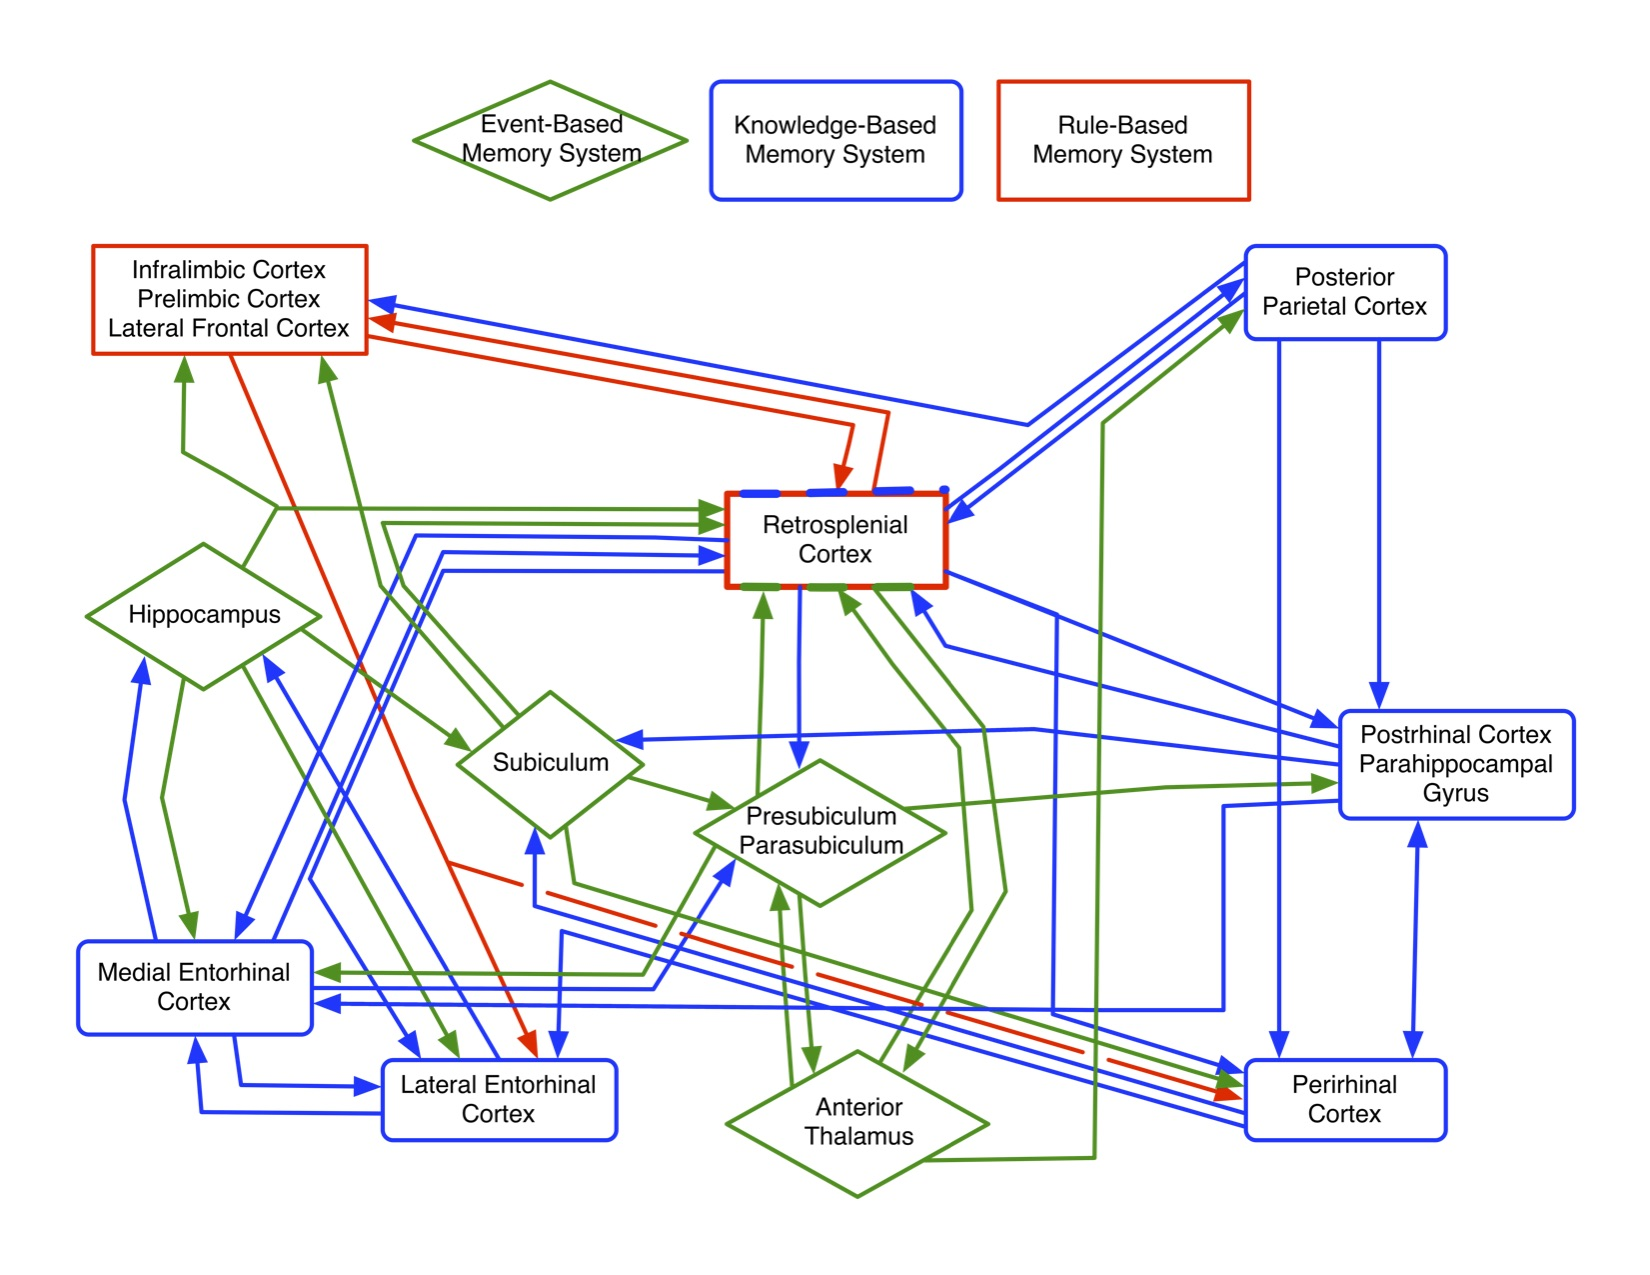
\includegraphics[width=.99\textwidth]{FIGURE1.jpg}
\centering
\begin{singlespace}
\caption{\textit{Neural networks involved in processing the spatial attribute within the event-based memory system, the knowledge-based memory system, and rule-based memory system. Particular attention should be paid to the interactive nature of these neural networks for spatial processing. These interactions are possible given the rich anatomical connectivity among these brain regions.}}
\label{fig1}
\end{singlespace}
\end{figure*}

At a psychological level, the event-based memory system subserves transient spatial representations of incoming data concerning present inputs, with an emphasis upon data and events that are personal or egocentric and occur within specific contexts. The emphasis of the event-based memory system is on the processing of current information that is novel. The event-based memory system is emphasized during the initial phases of learning, and will continue to be greatly important even after learning, so long as behavioral situations require unique or novel trial information need to be processed or remembered. This system is somewhat comparable to episodic memory and some aspects of declarative memory \parencite{Squire2004b,Squire1992b, Tulving}.

The knowledge-based memory system subserves more long lasting, permanent representations of already encoded spatial information in long-term memory. Knowledge-based memory can be conceptualized of as general spatial knowledge. As such, the knowledge-based memory system is of greater importance once a task has been learned, so long as the behavioral situation is both invariant and familiar. Within the knowledge-based memory system, the organization of the spatial attribute is organized as a set of interacting cognitive maps and their interactions that are unique for each memory \parencite{Hunsaker2013c,Kesner2013e}.

The rule-based memory system integrates spatial information from both the event-based and knowledge-based memory systems and applies rules and strategies that are necessary to guide subsequent action. In most situations, one would expect that all three systems with a varying proportion of involvement to provide behaviorally relevant contributions to spatial learning and memory processing \parencite{Kesner2013e,Kesner1998c}. 

Importantly, these event-based, knowledge-based, and rule-based memory systems are composed of the same attributes of memory. A spatial attribute within this attribute framework includes mnemonic representations of places or relationships among places. The spatial attribute is exemplified by the ability to encode and retrieve spatial maps and to localize stimuli in external space. Memory representations of the spatial attribute are further subdivided into specific features including allocentric spatial distance, egocentric spatial distance, allocentric direction, egocentric direction, metric and topological space, spatial location, and spatial context. In addition, there are specific spatial features associated with spatial navigation such as head direction and path integration \parencite{Hunsaker2013c,Kesner1998c}. 

Within each system, information related to the spatial attribute is differentially processed based on the operational characteristics of each memory system. For the event-based memory system, specific processes involve a) selective filtering or attenuation of interference of temporary memory representations of new information and is labeled pattern separation, b) encoding of new information, c) short-term and intermediate-term memory for new information, c) the establishment of arbitrary associations, d) consolidation or elaborative rehearsal of new information, and e) retrieval of new information based on flexibility, action, and pattern completion \parencite{Kesner2013e,Kesner1998c}. 

For the knowledge-based memory system, specific processes include a) encoding of new information, b) selective attention and selective filtering associated with permanent memory representations of familiar information, c) perceptual memory and d) consolidation and long-term memory storage partly based on arbitrary and/or pattern associations, and e) retrieval of familiar information based on flexibility and action \parencite{Kesner2013a}.

For the rule-based memory system, information is processed through the integration of information from the event-based and knowledge-based memory systems for the use of major processes that include the selection of strategies and rules for maintaining or manipulating information for subsequent action as well as \textit{short-term or working memory} for new and familiar information \parencite{Kesner2011a,Churchwell2011a,Kesner2000}. 

On a neurobiological level, it has been demonstrated that for the event-based memory system, the hippocampus is central to memory for spatial and spatial-context information; as well as spatial navigation. For the knowledge-based memory system, it has been demonstrated that the posterior parietal cortex (PPC) is central to memory for spatial attribute information. For the rule-based memory system, it has been demonstrated that the prelimbic and infralimbic cortices (PL-IL) are central to memory for spatial attribute information (For more details \textit{cf}., \cite{Kesner2011a,Churchwell2011a,Kesner2013a,Kesner1989,Kesner1998c,Kesner2000, Kesner2002,Kesner1987a,Kesner1989b,Kesner1996}.)

\section{Spatial attribute: Event-based memory system}
\subsection{Simplistic view of the hippocampus wiring diagram}

%NEED A NAIVE HIPPOCAMPUS FIGURE HERE
\begin{figure*}[htp!]
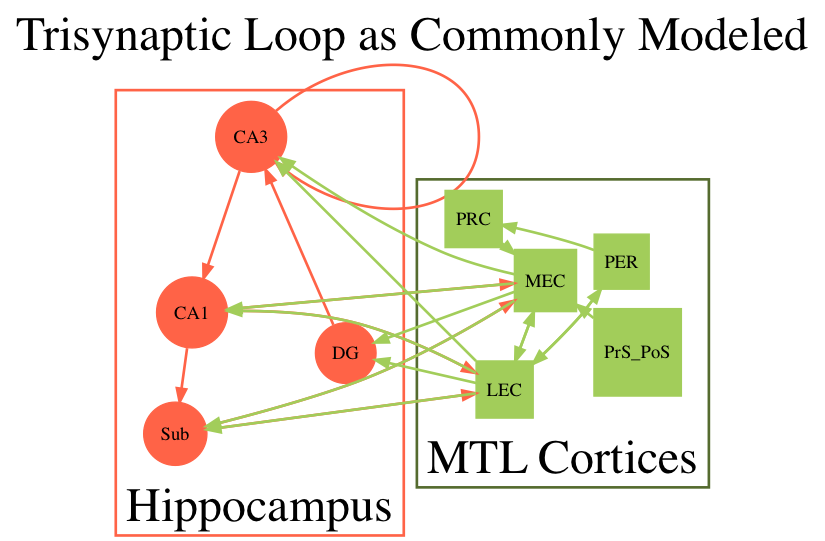
\includegraphics[width=.99\textwidth]{Simple.png}
\centering
\begin{singlespace}
\caption{\textit{Diagram of the simplified trisynaptic loop often used in simulations of hippocampus function. This is a convenient simplification for hypothesis testing, but the reality of hippocampus wiring is much more complex.}}
\label{fig2}
\end{singlespace}
\end{figure*}

Traditionally, the hippocampus is described in terms of the trisynaptic loop (Fig~\ref{fig2}). This loop refers to inputs from layer II of the medial and lateral entorhinal cortices entering the hippocampus via the perforant path, which synapses in the molecular layer of the DG. The DG granule cells project via the mossy fibers to the stratum lucida of CA3. CA3 then projects to CA1 via the Schaffer collaterals, which synapse in the stratum radiatum. CA1 then serves as the primary output of the hippocampus, projecting to the subiculum and the deep layers (primarily layer V) of the entorhinal cortex. 

This is a convenient description of the hippocampus, and it has informed numerous computational models of hippocampus function (\textit{cf}., \cite{Rolls1989a,Rolls1996a}). Despite this utility, there are increasing evidence described below that suggest the complexity within the hippocampus needs to be emphasized in order to elucidate the nature of hippocampus processing of spatial and nonspatial information \parencite{Hunsaker2013c}. This is particularly important as the functions of the direct perforant path into CA1 and CA3 have been demonstrated to be important for spatial and nonspatial information processing \parencite{Hunsaker2007c} and the cells within the hilus have been shown to participate in pattern separation-related processes \parencite{Neunuebel2014a}.

\subsection{A more accurate view of the hippocampus wiring diagram}

% Figure 3 NOT SO NAIVE HIPPOCAMPUS
\begin{figure*}[htp!]
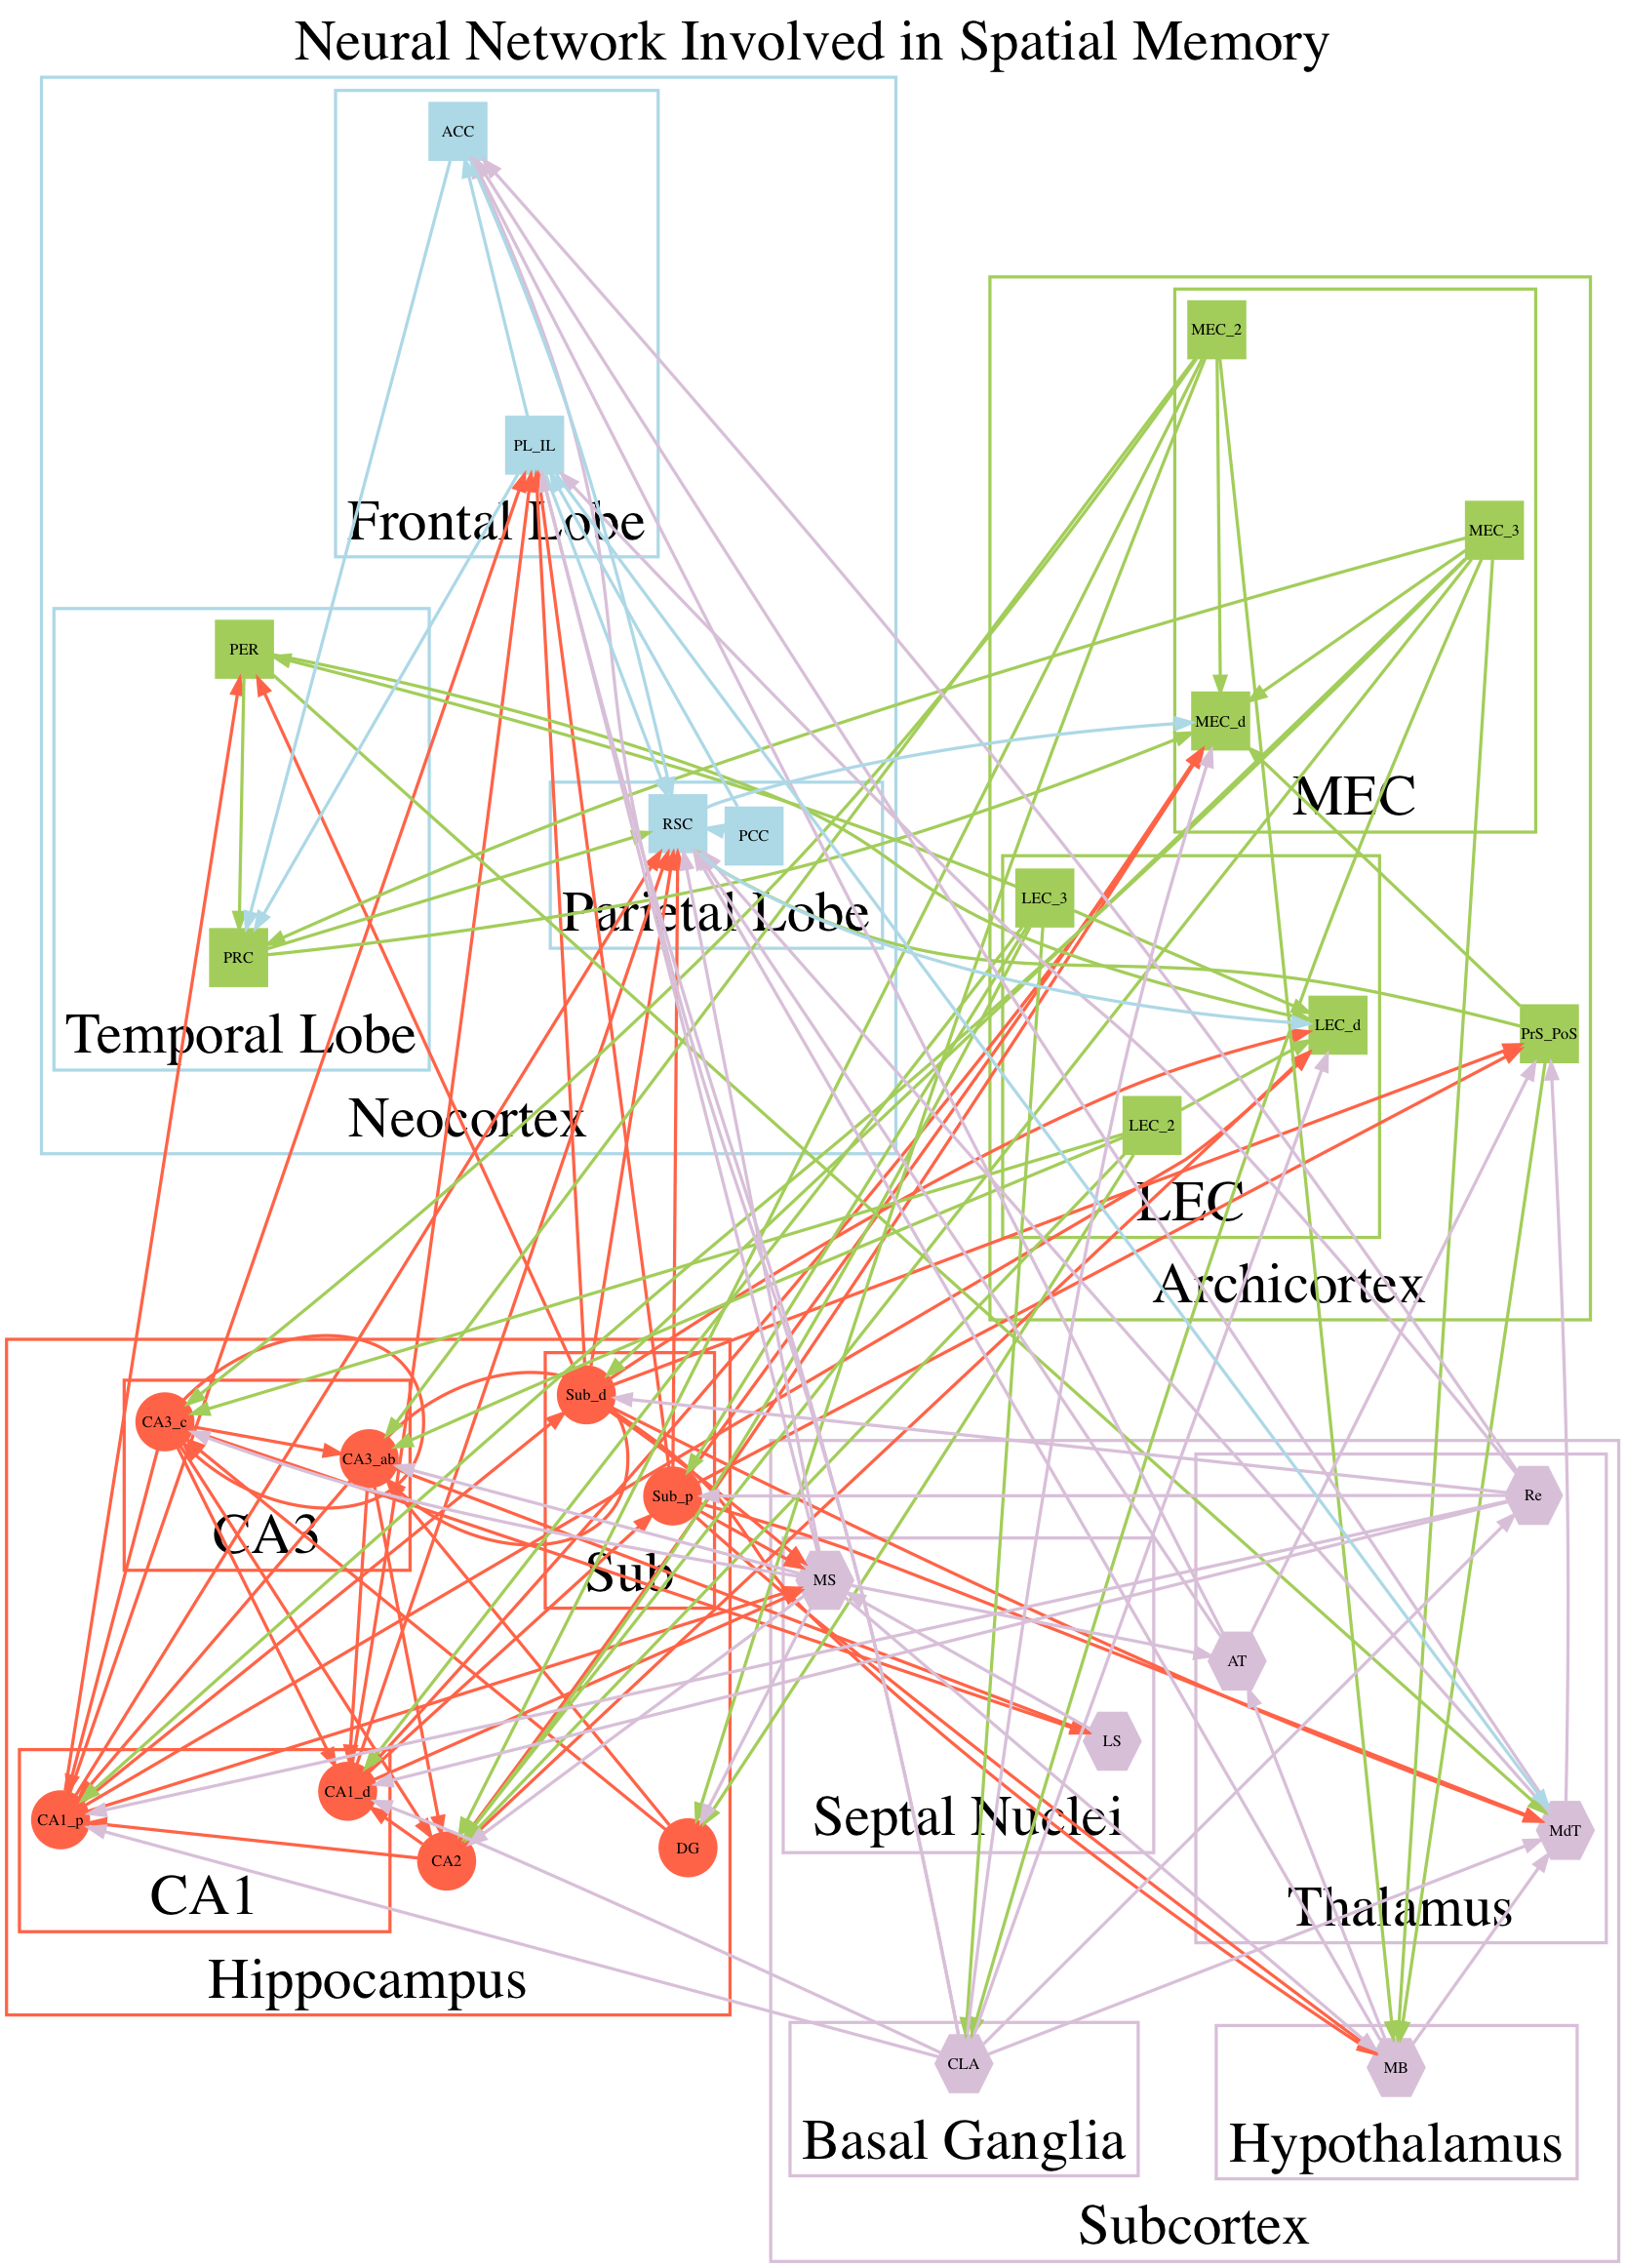
\includegraphics[width=.99\textwidth]{Complicated.png}
\centering
\begin{singlespace}
\caption{\textit{Hippocampal circuitry}}
\label{fig3}
\end{singlespace}
\end{figure*}


A more accurate representation of the hippocampus wiring diagram as well as a more accurate representation of hippocampus interactivity with the rest of the brain is depicted in Fig~\ref{fig3}.

\subsubsection{Dentate gyrus}
The medial and lateral perforant path inputs from layer II of the entorhinal cortex to the DG synapse in different sublayers of the molecular layer. The medial perforant path synapses are located in the inner molecular layer of the DG, whereas the lateral perforant path synapses in the outer molecular layer. The dentate gyrus projects via the mossy fibers to the stratum lucida of CA3, but these mossy fibers also make \textit{en passant} synapses in the polymorphic layer (or hilus) onto mossy cells and local interneuron populations. The mossy cells and local interneurons provide inhibitory feedback into the DG. Similarly, the pyramidal cells in CA3c (in the rat) have projections back into the hilus onto mossy cells and interneurons, as well as limited synapses back onto DG granule cells \parencite{Kesner2013, hunsaker2008role}.

\subsubsection{CA3}
Unlike the traditional diagrams that treat CA3 as a unitary entity, the anatomy suggests at least 3 distinct subregions: CA3c which is surrounded by the blades of the dentate gyrus, CA3b which refers to the area of CA3 just lateral to the dentate gyrus and contains approximately half the bend observed in CA3. CA3a refers to the area between CA2 and CA3b. 

What is common to all subregions within CA3 is that they receive mossy fiber inputs from the DG (as quantified by Timm's staining), send Schaffer collaterals into CA1 and commissural fibers to the contralateral hippocampus, and project via the fimbria and precommisural fornix to the lateral septal nuclei. In addition to the mossy fiber inputs from the DG, CA3 also receives direct entorhinal inputs via the perforant path. Similarly to the DG, the medial perforant path synapses more proximally within the stratum lacunosum-moleculare than the lateral perforant path. Interestingly, it has been demonstrated that the perforant path synapses onto CA3 fire on average 1-2 ms prior to dDG activation to the same stimulus. CA3a and CA3b additionally demonstrate a robust recurrent collateral circuitry.

What makes these areas unique is the CA3c does not receive recurrent collateral synapses from CA3a or CA3b, and thus may process input patterns in relative isolation to these regions. CA3c does, however, maintain projections to CA1 via the Schaffer collaterals as well as projections to the septum and diagonal band of broca via the precommisural fornix. Additionally CA3c projects into the polymorphic layer in the hilus and thus may form a sort of feedback loop with the DG. 

\subsubsection{CA2}
Although not much is known about CA2, it is becoming a focus of study in recent years. It has been shown that CA2 receives a direct perforant path projection from layers II and III of the entorhinal cortex and that these CA2 synapses activate even before those in CA3. CA2 receives no mossy fiber projections (indicated by a negative Timm's staining). CA2 also receives a Shaffer collateral input from CA3. CA2 projects to CA1, but primarily to the strata oriens, rather than to the stratum radiatum like CA1. Also, CA2 projects directly to layer II and layer V of the entorhinal cortex \parencite{Rowland2013a}.

\subsubsection{CA1}
CA1, similar to CA3, has something of an inhomogeneous structure. The proximal portion of CA1 (that which abuts CA2) primarily receives projections from the lateral perforant path, whereas the distal CA1 (adjacent to the subiculum), receives primarily medial perforant path innervation. Distinct from the other hippocampus subregions, the perforant path inputs to CA1 are primarily from layer III of the entorhinal cortex, with only small inputs from 'cell islands' in layer II of the entorhinal cortex. 

The entire extent of CA1 receives Schaffer collateral and commissural inputs from CA3 that synapse in the stratum radiatum and a projection from CA2 that synapses in the stratum oriens. Also distinct from the other hippocampus subregions, a direct projection from the perirhinal cortex has been identified in CA1.

CA1 sends projections via the fornix to the medial septum and the rest of the Papez circuit (\textit{e.g.}, anterior thalamus, septal nuclei, mammillary bodies). Additionally, CA1 projects to layer V of the entorhinal cortex as the primary output of the hippocampus, as well as to the subiculum. Interestingly, it has been shown that CA1 projections to the subiculum are topographically organized, such that proximal CA1 projects to distal subiculum (far from CA1) and distal CA1 projects to the proximal siubiculum. Some outputs (in rats) from CA1 also travel along the temporoammonic pathway toward the PL-IL and retrosplenial cortex \parencite{Jay1991a}.

\subsubsection{Subiculum}
Although the subiculum is often excluded as a portion of the hippocampus proper, it is included here as it has extensive connectivity with CA1 and the fact that the subiculum receives direct perforant path projections from the entorhinal cortex. Similar to CA1, the subiculum receives a topographically separated perforant path input from entorhinal cortex layer III. The proximal subiculum receives medial perforant path inputs similar to the adjacent distal CA1. The distal subiculum receives primarily lateral perforant path inputs similar to proximal CA1. This topographical segregation of inputs is also true for the CA1 projections into the subiculum, with the distal CA1 projecting to the proximal subiculum (preserving medial perforant path inputs) and the proximal CA1 projects to the distal subiculum (preserving lateral perforant path inputs). 

The outputs of the subiculum are similar to CA1, projecting to the deep layers of the entorhinal cortex as well as through the fornix to structures along the Papez circuit and hypothalamus. The subiculum also has a unique projection to the amygdala as well as pre- and parasubicular cortices.

\subsection{Processes Within the Event Based Memory System}
\subsubsection{Short-term working memory for spatial location}
The most comprehensive set of data that demonstrate the role of the event-based memory system for short term or working memory processing come from paradigms such as delay nonmatch-to-sample, delayed conditional discrimination, continuous recognition memory of single or lists of items, and recognition memory based on exploratory information and detection of novelty. The results of experiments using these paradigms to measure short-term or working memory for spatial information clearly demonstrate that there are severe impairments for rats with bilateral hippocampal damage \parencite{Kesner1990c, Olton1983a, Olton1986a, Lee2003, Kesner2011a}.

With respect to allocentric spatial distance, egocentric spatial distance, and spatial location, it has been shown in rats with bilateral hippocampal damage that there are severe deficits in short-term memory for these spatial features \parencite{Long1996a}. These findings provide support for a potential role for place cells (cells that increase their firing rate when an animal is located in a specific spatial location) within the hippocampus of rats being involved for spatial memory \parencite{Kubie1983a, McNaughton1983a, OKeefe1987a, OKeefe1978a}. It has been shown that hippocampus lesions produce deficits for a continuous spatial recognition task \parencite{Jackson-Smith1993a}. Short-term memory for the spatial direction feature has been investigated using a delayed matching-to-sample task for assessing memory for direction in rats. The results of this experiment demonstrated that hippocampal lesions disrupt memory for direction \parencite{DeCoteau2004a}, and there is a suggestion that this sense of direction in rats is impaired after lesions to the dorsal subiculum \parencite{Potvin2007a}. Together, these spatial short-term memory representations within the hippocampus are likely important to initiate downstream consolidation processes as necessary and spatial short-term memory representations within the PL-IL might provide relevant signals to initiate a retrieval, action, or strategy selection process. Thus, in general, the hippocampus represents within short-term memory some of the spatial features associated with the spatial attribute (\textit{cf.}, \cite{Kesner2002,Kesner2013e}).

Based on a subregional analysis of hippocampal function, it appears that different subregions subserve differential roles in spatial processing of short-term memory (\textit{cf.}, \cite{Kesner2004b}). For example, using a paradigm developed by \textcite{Poucet1989a}, rats with dorsal DG (dDG), dorsal CA3 (dCA3) or dorsal CA1 (dCA1) lesions were tested for the detection of a novel spatial configuration of familiar objects \parencite{Lee2005b, Lee2005c}. They found was that the dDG and dCA3 were necessary for the rapid formation of spatial memory and lesions to either the dDG or dCA3 subregions of the hippocampus resulted in profound deficits for re-exploration of a spatial change in the arrangement of familiar objects. However, dCA1 showed a much more modest impairment, suggesting a dissociation in spatial novelty detection across hippocampus subregions. 

To test the hypothesis that the medial perforant path input into dDG, dCA3 or dCA1 mediates spatial information via activation of NMDA receptors, rats received direct infusions of AP5 (an NMDA receptor antagonist) into the dDG, dCA3, or dCA1 and were tested for the detection of a novel spatial configuration of familiar objects and the detection of a novel visual object change using the same paradigm mentioned above. The results indicated that AP5 infusions into the dCA3 disrupted both novelty detection of a spatial location and a visual object, whereas AP5 infusions into the dDG or dCA1 disrupted novelty detection of a spatial location, but not the detection of a novel object \parencite{Hunsaker2007c}. More to the point, in dCA3, disrupting plasticity in the lateral perforant path using naloxone infusions (blocking nonspatial information) also disrupted spatial memory. In this case, it appears the medial perforant path and the recurrent collateral system in dCA3 were either actively maintaining the spatial and non-spatial information as a single behavioral episode in the network over the three minute intersession interval or else that the rich spatial context available to the rats upon the test session was sufficient to guide retrieval of the previous experience to guide test performance, reflective of event-based memory processing. In the dDG and dCA1, in the absence of recurrent circuitry, appeared to be acting directly upon the spatially rich medial perforant path inputs to retrieve the spatial information needed to perform the test. It is of interest that the dDG and dCA1, as opposed to dCA3, did not appear to retrieve the overall behavioral episode in this case to guide retrieval, only the spatial aspects of the experience. 

Using different methods, \textcite{Lee2004d} and \textcite{Neunuebel2014a} showed physiologically that plasticity mechanisms in dDG and dCA3 showed altered cellular firing only when animals encountered novel spatial configurations of familiar cues for the first time. Specifically, rats were trained to circle clockwise on a ring track whose surface was composed of four textural cues (local cues). The ring track was positioned in the center of a closed area in which various visual landmarks were prominently displayed on the walls. To produce a novel cue configuration in the environment, distal landmarks and local cues on the track were rotated in opposite directions (distal landmarks were rotated clockwise and local cues were rotated counterclockwise by equal amounts). It is well known that pyramidal and granule cells in the hippocampus fire when the animal occupies a certain location of space, known as the 'place field' of the cell. Mehta and colleagues \cite{Mehta1997a, Mehta2000a} showed that the location of the dCA1 place field (center of mass of the place field) changed over time, by shifting backward opposite to the direction of rat's motion, in a familiar environment as the animal repeatedly experienced the environment. When the rats encountered the changed cue configurations for the first time in the \textcite{Lee2004d} experiment, the dCA3 place fields shifted their locations backwards prominently compared to the place fields in dCA1. In the \textcite{Neunuebel2014a} experiment, they found that the dDG place fields fractionated at even the slightest changes to the environment. However, prominent shifts were not observed in dCA3 from day 2 onwards (dCA1 place fields exhibited that property starting at day 3). 

This triple dissociation in the time course of plasticity between the dDG, dCA3, and dCA1 place fields suggests that dDG reacts immediately to any change in the environment (reflecting rapid pattern separation processes), followed by dCA3 which reacts more rapidly to any changed components in the environment relative to dCA1, presumably to incorporate the newly experiences spatial information into an existing event-based short-term memory system or contribute to a new representation of the environment mediated by an event-based short-term memory system if changes are significant \parencite{Neunuebel2014a}. Interestingly, in the very short term, it appears that the dCA3 initially recalls previously experienced activity patterns rather than showing fracturing of place fields as recorded in the dDG. However, within only a matter of minutes dCA3 activity begins to reflect the patterns observed in the dDG. Dorsal CA1 appears to be performing a similar function as dCA3, but within an intermediate-term event-based memory system as demonstrated by the different time course than dDG and dCA3, suggesting that the representation of the behavioral episode in dCA1 is processed on a longer timescale than in dCA3. These data suggest that in some cases dCA3 processes information and communicates that information to dCA1 via the Schaffer collateral projections for comparison with medial perforant path inputs. 

\textcite{Hampson1993a} recorded ensembles of dCA3 and dCA1 neurons during a spatial delay non-match to sample task and found a similar pattern of results. They found cells responsive to spatial location, nonspatial attributes of the task, and cells responsive to conjunctions of spatial and nonspatial information (which they called \textit{conjunctive cells}). Fairly often they found activity in dCA1 to be highly correlated to activity in dCA3 at earlier timepoints (meaning the CA1 activity at time interval 1 or 2 was highly correlated with CA3 activity at time 0), suggesting information was preserved when it was transferred from dCA3 to dCA1. 

With respect to allocentric spatial distance, egocentric spatial distance, and spatial location, it has been shown that bilateral hippocampal damage in rats produces severe deficits in short-term memory for these features \parencite{Long1996a}, consistent with the activity of place cells within the rodent hippocampus \parencite{Kesner1990c, Olton1983a, Olton1986a, Lee2003, Kesner2011a, OKeefe1978a}

\subsubsection{Consolidation}
The hippocampus also plays a role in the acquisition or learning of new spatial information requiring the consolidation of spatial attributes. Spatial navigation tasks in a water maze, dry-land version of the water maze, and inhibitory avoidance tasks have been used to demonstrate this. In these tasks, rats with hippocampal lesions show dramatic impairments \parencite{OKeefe1978a, Morris1982a, Kesner1990c}. Furthermore, post-trial inactivation of hippocampal function using electrical brain stimulation results in time-dependent memory impairments \parencite{Kesner1974a}. These effects suggest the hippocampus is involved in short-term consolidation. This is a reasonable hypothesis because the memory gradients are short, within minutes to a few hours. Long-term, temporally graded functions (2-4 weeks) have been observed for previously learned spatial discriminations, but are observed primarily following entorhinal cortex but not hippocampus lesions \parencite{Cho1995b, Cho1995c}. Long term memory gradients following hippocampal damage have been reported in contextual fear conditioning \parencite{Kim1992a}, but follow up studies bring into question whether such gradients can truly be measured reliably \parencite{Maren1996a, Weisend1996a}. 	

As such, it is possible that short-term consolidation gradients derive from hippocampal dysfunction, whereas entorhinal cortex dysfunction is necessary to produce the consolidation gradients associated with long-term retrograde amnesia (\textit{i.e.}, hipocampus participates in short term consolidation and the entorhinal cortex participates in long term consolidation; \cite{Cho1995b, Cho1995c}). Also, it is important to note that the consolidation process could also involve backprojections from the entorhinal and perirhinal cortex to neocortical areas which could then could provide information useful to the neocortex in the building of new spatial representations in the multimodal and unimodal association cortical areas as part of the knowledge-based and rule-based systems \parencite{Lavenex2000a, Preston2005}. To date it is still unknown whether the hippocampus promotes the transfer of spatial information to the knowledge and rule-based systems or whether the hippocampus promotes the consolidation of already processed information in the knowledge and rule-based systems.

\subsubsection{Pattern Separation}
Single pyramidal and granule cells within the hippocampus are activated by most sensory inputs, including vestibular, olfactory, visual, auditory, and somatosensory as well as higher-order integration of sensory stimuli \parencite{Eichenbaum1993b}. Whether these sensory inputs have a memory representation within the hippocampus remains a matter of active debate. A putative role for the hippocampus in processing all sensory information may be to process sensory markers to anchor spatial location, so that the hippocampus can more efficiently mediate spatial information. Possibly, that one of the main process functions of the hippocampus is to encode and separate spatial events from each other. A function such as this would ensure that incoming, new highly processed sensory information is organized within the hippocampus to enhance the possibility of remembering and temporarily storing one spatial location as separate from every other place. The process proposed to underlie this process is called pattern separation of event information. Pattern separation processes make it so that spatial events can be separated from each other and spatial interference is reduced. This process is akin to the idea that the hippocampus is involved in orthogonalization of sensory input information \parencite{Hunsaker2007c,hunsaker2013operation, Kesner2002, Kesner2013e, Rolls1989a}, in representational differentiation \parencite{Gluck1997b}, and/or indirectly by flexible utilization of relationships \parencite{Eichenbaum1993b}. 
	
As previously described by \textcite{Kesner2013e} and \textcite{Gilbert1998a, Gilbert2001a}, to assess pattern separation processes rats were trained in a spatial memory task. Rats were required to remember a spatial location dependent upon the distance between the study phase object and an object used as a foil. More specifically, during the study phase an object which covers a baited food well was randomly positioned in one of fifteen possible spatial locations on a cheese board. Rats exited a start box and displaced the object in order to receive a food award and were then returned to the start box. On the ensuing test phase rats were allowed to choose between two objects which were identical to the study phase object. One object was baited and positioned in the previous study phase location (correct choice), the other (foil) was unbaited and placed in a different location (incorrect choice). Five distances (min =15 cm, 37.5 cm, 60 cm, 82.5 cm, max =105 cm) were randomly used to separate the foil from the correct object. Following the establishment of a criterion of 75\% correct averaged across all separation distances, rats were given either large (dorsal and ventral) hippocampal or cortical control lesions dorsal to the dorsal hippocampus. Following recovery from surgery the rats were retested. The results indicate that whereas control rats matched their pre-surgery performance for all spatial distances, hippocampal lesioned rats displayed impairments for short (15 cm-37.5 cm) and medium (60 cm) spatial separations, but performed as well as controls when the spatial separation was long (82.5-105 cm). The fact that the hippocampal lesioned group was able to perform the task well at large separations indicates that the deficits observed at the shorter separations were not the result of an inability to remember the rule. The results suggest that the hippocampus may serve to separate incoming spatial information into patterns or categories by temporarily storing one place as separate from another place (this is described in more detail by \cite{hunsaker2013operation} and \cite{OReilly2001a}).

As a control, it was demonstrated that ability to remember the longest distances was not based on an egocentric response strategy, because if the study phase was presented on one side of the cheese board and the test originated on the opposite side, the hippocampal lesioned rats still performed the long distances without difficulty. Furthermore, the hippocampal lesioned group had no difficulty discriminating between two short distances. It is clear that in this task it is necessary to separate one spatial location from another spatial location. Hippocampal lesioned rats cannot separate these spatial locations very well, so that they can perform the task only when the spatial locations are far apart \parencite{Gilbert1998a}. In follow-up experiments, rats with dDG lesions were tested in the same pattern separation experiment described above. The results indicated that the DG lesioned rats were significantly impaired at short spatial separations; however, during the choice phase performance of dDG lesioned animals increased as a function of greater spatial separation between the correct and foil objects. The performance of rats with dDG lesions matched control rats at the largest spatial separation. The graded nature of the impairment and the significant linear improvement in performance as a function of increased separation illustrate a deficit in pattern separation (\textit{cf.}, \cite{hunsaker2013operation}). Based on these results, it was concluded that lesions of the dDG decrease the efficiency of spatial pattern separation, which results in impairments on trials with increased spatial proximity and increased spatial similarity among working memory representations \parencite{Gilbert2001a}.

Thus, the dDG appears to function in a way that encodes and separates events in space, thereby producing spatial pattern separation (\textit{cf.}, \cite{Rolls1996a, Rolls2006b}). Spatial pattern separation ensures that new highly processed sensory information is organized within the hippocampus, which in turn enhances the possibility of efficiently encoding and easily remembering one spatial location as separate from another without catastrophic interference.

Based on the observation that neurogenesis occurs in the DG and that new DG granule cells are generated across time, it is possible that the dDG mediates spatial pattern separation as well as generates patterns of episodic memories within remote memory (\textit{i.e.}, mnemonic pattern separation; \cite{Aimone2006a, hunsaker2013operation}). It has been shown in mice that low-dose x-irradiation produces a loss of newly born dDG cells and impairments in spatial learning in a delayed non-matching-to-place task in the radial arm maze. Specifically, there were specific impairments for arms which were presented with very little spatial separation, but no deficits were observed when the arms were presented farther apart \parencite{Clelland2009a}. This distinction between deficits with high interference but spared function with low interference provides evidence for a spatial pattern separation deficit. 

Another study in mice provided evidence that the disruption of neurogenesis using lentivirus expression of a dominant negative version of Wnt produced a loss of newly born dDG cells.  This manipulation was sufficient to disrupt performance in an associative object-in-place task with different spatial separations as a function of the degree of separation, again suggesting a spatial pattern separation deficit \parencite{Clelland2009a}. In a more recent study by \textcite{kesner2014role}, it was shown that blocking DNA methyltransferace 1-c in mice reduced neurogenesis and impaired spatial pattern separation relative to controls, using the \textcite{Goodrich-Hunsaker2005a} spatial pattern separation task (described in detail in the next paragraph). Given these data, neurogenesis in the dDG appears to  contribute to the operation of spatial pattern separation. Thus, spatial pattern separation serves a pivotal role in the acquisition of new spatial information and there is a good possibility that the dDG may be the subregion responsible for the impairments in the various tasks described above.

What was left was to study the question of whether spatial pattern separation play a role in novelty detection of changes in spatial distance based on metric changes. Using a modified version of an exploratory paradigm described by \textcite{Poucet1989a}, rats with dorsal hippocampus, dDG, dCA3, or dCA1 lesions were tested on tasks involving either metric spatial or topological spatial manipulations. In the metric manipulation, a rat was allowed to explore two different visual objects that were separated by a specific distance on a cheeseboard maze. After habituation to the objects and their locations, the metric spatial distance between the two objects was manipulated so the two objects were either closer together or further apart than during the habituation phase. The time the rat spent exploring each object was recorded. In the topological condition, rats were allowed to explore four different visual objects that were positioned in a square on the cheeseboard maze. After habituation, the locations of two of the objects were transposed and the time the rat spent exploring each object was recorded. The results showed that dorsal hippocampus and dDG lesions impaired detection of the metric manipulation, but not the topological manipulation. In contrast, dCA3 and dCA1 lesions did not impair performance after either the metric or the topological manipulation. The results suggest that granule neurons in the dDG may be involved in processing spatial information on a metric scale but may not be required for representing topological space \parencite{goodrich2008interactions, Goodrich-Hunsaker2005a}.

Does spatial pattern separation based on spatial interference play a role in the acquisition (consolidation) hippocampal dependent tasks? Because rats are started in different locations in the standard water maze task, there is likely that there may be high levels of interference among similar and overlapping spatial patterns. The observation that hippocampal lesioned rats are impaired in learning and subsequent consolidation of important spatial information in this task can be attributed  to the difficulty of separating spatial patterns, resulting in enhanced spatial interference. \textcite{Eichenbaum1990a} supported this idea when they demonstrated that when fimbria-fornix lesioned rats are trained on the water maze task from only a single starting position (less spatial interference) the learning deficits are very small to absent, whereas training from multiple starting positions resulted in deficits. In a similar study it was shown that total hippocampal lesioned rats learned or consolidated rather readily that only a single spatial location was correct on an 8 arm maze \parencite{Hunt1994a}. 

\textcite{McDonald1995a} demonstrated similar effects using a place preference procedure using an eight arm maze. They placed food at the end of one arm and no food at the end of another arm. In a preference test normal rats preferred the arm that contained the food. Fornix lesioned rats acquired the place preference task as quickly as controls if the arm locations were opposite each other, but the fornix lesioned rats showed difficulty in learning the task if the rewarded locations were adjacent to each other. Clearly, there would be greater spatial interference when the spatial locations are adjacent to each other rather than far apart. Thus, spatial pattern separation plays a role in the acquisition of new spatial information. A similar study by \textcite{morris2012selective} obtained similar results with dDG lesions, and another study from \textcite{Potvin2009a} demonstrated that the dorsal subiculum may be involved for overcoming interference among environmental cues associated with this task.

\subsubsection{Spatial context-pattern separation for color of the environment}
It has been suggested that the hippocampus processes context based on background cues, such as floor or overall environmental color \parencite{Jeffery2003a, Norman2004a}. \textcite{kesner2016dentate} designed an experiment in order to test whether the dDG plays an important role in processing of context based on colors and whether it is possible to generate a pattern separation effect based on different shades of black and white. Four shades of color boxes were constructed: white, light gray, dark gray and black, and four shaded inserts were constructed to fit inside each box: white, light gray, dark gray and black. The inserts were constructed to cover half of each box, such that the two sides of each box had different shades of color. On the test day during the study phase dDG lesioned rats and controls were placed in one of the colored boxes, with a colored insert that was different than the color of the box for a 5 min period. Then the rat was placed into its home cage for ten minutes. During the 10 min retention interval either the insert or box color was changed to generate the context of the test phase. The study phase had a duration of 5 min. Context exploration was measured throughout the study and the test phase by the number of observed rearing events against the wall each subject exhibited on the insert side and the box side (the side without the insert). Each rearing event constituted removing both front paws from the ground. Each subject was tested for 12 days, using the number of rearing events to measure novelty detection. Each experimental day was followed by a rest day or a 48 hour break period, taking a total of 24 days for each rat to complete the task. 

Three context gradient levels were measured, taking the difference of the novel color (introduced during the test phase) and the familiar from the study phase with Level 1 a context gradient was a slight color change-white to light gray, light gray to dark gray, dark gray to black, or the reverse of any of the former. Level 2 with a context was a medium color change-white to dark gray, light gray to black or the reverse of any of the former. Level 3 with a context that was the maximum color change-white to black or the reverse. Each subject completed four trials at level 1, level 2 and level 3 context gradient transitions. These levels were used to establish the degree to which subjects noticed the context change. The results of the experiment indicates that control rats displayed a color pattern separation effect across levels of separation of context (shades of color), but the dDG lesioned rats did not display a color pattern separation across levels 1, 2, and 3 \parencite{kesner2016dentate}. In other words, lesioning the dDG was sufficient to disrupt pattern separation for the color of the environment. To support the idea that rats in this task primarily process recognition for color as the primary contextual cue, it can be shown that during the study phase there is a preference for the darker color for both groups, but during the test or recognition memory phase there is no preference for the darker color for both groups, suggesting that the dDG plays an important role in context recognition for colors by reducing interference between shades of color.

\subsubsection{Retrieval of spatial information}
Even though it has been proposed that the hippocampus also plays an important role in retrieval of new information \parencite{Hirsh1974a}, there are only limited data supporting a retrieval function for the hippocampus. Eichenbaum and colleagues developed transitivity tasks to show that rats with hippocampal lesions are impaired for retrieving novel information, suggesting a lack of flexibility in solving new problems (\textit{cf.}, \cite{Bunsey1996b}). However, other studies that have tested hippocampal lesioned rats have shown normal transfer to novel tasks, suggesting flexible use of information to solve new problems \parencite{Jackson-Smith1993a, DeCoteau1997a, Cho1995b, Walker1984a}. Thus, there is some, albeit limited, support for a hippocampus mediated retrieval function. What has been shown is that isolating CA1, but not CA3 subcortical efferents result in retrieval deficits on a modified Hebb-Williams maze \parencite{hunsaker2008double}, but it remains unknown whether this effect reflects hippocampus-dependent retrieval processes or a disruption to retrieval processes initiated by structures along the Papez circuit by depriving them of hippocampus inputs via the fimbria/fornix pathways.

\subsubsection{Temporal order memory for spatial locations}
\textcite{Estes1986a} summarized human experimental data demonstrating that there are fewer errors for distinguishing items that are far apart in a sequence than those that are temporally adjacent (referring to the order in which they occurred). Many studies have also shown that order judgments improve as the number of intervening items between test items in a sequence increases \parencite{Banks1978, Chiba1994a, Madsen1995a}. This phenomenon is referred to as a temporal distance effect (sometimes referred to as a temporal pattern separation effect; \textit{cf.}, \cite{hunsaker2013operation, Kesner2004b, kesner2010temporal}). The temporal distance effect is assumed to occur because there is more interference for temporally proximal events than for temporally distant events \parencite{Kesner1998c, Kesner2002, Kesner2013e}. 

Building upon these earlier findings, \textcite{Gilbert2001a} tested memory for the temporal order of spatial locations in a one-trial sequence learning paradigm in rodents. In this task, each rat was given one daily trial consisting of a sample phase followed by a choice phase. During the sample phase, the animal visited each arm of an 8-arm radial maze once in a randomly predetermined order and was given a reward at the end of each arm. The choice phase began immediately following the presentation of the final arm in the sequence. In the choice phase, two arms were opened simultaneously and the animal was allowed to choose between the arms. To obtain a food reward, the animal had to enter the arm that occurred earlier in the sequence that it had just followed. Temporal separations of 0, 2, 4, and 6 were randomly selected for each choice phase. These values represented the number of arms in the sample phase that intervened between the arms that were to be used in the test phase. After reaching criterion, rats received dCA1 lesions. 

Following surgery, control rats matched their preoperative performance across all temporal separations. In contrast, rats with dCA1 lesions performed at chance across 0, 2, or 4 temporal separations and a little better than chance in the case of a separation of 6 items. The results suggest that the dCA1 subregion is involved in memory for spatial location as a function of temporal separation of spatial locations; lesions of the dCA1 decrease efficiency in temporal pattern separation. dCA1 lesioned rats cannot separate events across time, perhaps due to an inability to inhibit interference that may be associated with sequentially occurring events. The increase in temporal interference impairs the rat's ability to remember the order of specific spatial locations.

Using a different task designed to test memory for a sequence of spatial locations presented on a large, open environment, \cite{Hunsaker2008h, Hunsaker2008g} demonstrated that dorsal CA1, but not ventral CA1 or any other hippocampus subregion appeared to be involved for temporal ordering for spatial locations. In a follow up study \cite{Potvin2010a} replicated these findings using lesions of the dorsal subiculum, suggesting the dorsal subiculum works cooperatively with dorsal CA1 for temporal processing of spatial location information. 

\subsubsection{Spatial arbitrary associations}
Another function of the hippocampus and its subregions is to support the formation of arbitrary associations, particularly paired-associate learning \parencite{Eichenbaum1993b, OKeefe1978a}. A computational model from \textcite{Rolls1996a} suggested that the hippocampus, specifically the CA3 auto associative network, may be responsible for the formation of arbitrary associations (also \textit{cf.}, \cite{OReilly2001a}). In their example, information from posterior parietal cortex (PPC) regarding location may be associated with information from temporal cortex regarding object identity. This information reaches the  CA3 subregion of the hippocampus via the perforant path at which point CA3 binds these information streams into a single memory or behavioral episode, thus enabling the organism to remember an object and its location.

Our lab has designed a series of experiments to directly test the involvement of the hippocampus in spatial paired-associate learning \parencite{Gilbert2002a, Gilbert2003b}. In this task rats were trained on a successive discrimination go/no-go task to examine object-place paired associate learning. In this task rats with hippocampal lesions were severely impaired in learning object-place paired associations compared to control rats \parencite{Gilbert2002a}. In a second task rats were trained on a successive discrimination go/no-go task to examine odor-place paired-associate learning. In this task, the same procedure was used, except that rats need to learn that when an odor is presented in its paired location the rat should dig in sand mixed with the odor to receive a reward. Rats with hippocampal lesions were severely impaired relative to controls in learning odor-place paired-associations. Data from our laboratory using the above mentioned paradigms indicate that rats with dCA3 lesions are severely impaired in object-place and odor-place paired-associate learning. However, animals with dDG or dCA1 lesions learn the object-place and odor-place tasks as well as controls \parencite{Gilbert2003b}. These data support the hypothesis that dCA3, but not dDG or dCA1, support paired-associate learning when a stimulus is associated with a spatial location.

In another task rats were trained on a successive discrimination go/no-go task to examine odor-object paired-associate learning. In this task, the same procedure was used, except that rats need to learn that when an odor is presented in front of its paired object, the rat should dig in sand mixed with the odor to receive a reward. The results indicate that rats with hippocampal lesions acquire the odor-object task as quickly as controls \parencite{Gilbert2002a}. These data suggest that the hippocampus is clearly involved in paired-associate learning when a stimulus must be associated with a spatial location, but the hippocampus does not appear to be important when a spatial location is not a component of the paired-associate task. Support for this idea comes from a number of studies demonstrating that the hippocampus is not involved in arbitrary associations that involve odor-odor \parencite{Bunsey1993a, Li1999a}, odor-reward \parencite{Wood2004a}, and object-object associations \parencite{Cho1995b, Cho1995c, Murray1993a}).

It has also been demonstrated by \textcite{hunsaker2006role} that dCA3 is critical for learning object-place associations when the object and place are separated by a 10 second trace interval using a a successive discrimination go/no-go paradigm similar tot hat described above (object-trace-place task). In this experiment the rat was presented with an object in a start box for 5 seconds and then the object was removed for 10 seconds. The rat was then allowed to choose which of two locations marked with identical foil objects was associated with the object they had been presented. In this experiment both  dCA3 and dCA1 resulted in performance deficits. A separate experiment evaluated object-trace-odor learning. This experiment demonstrated that only dCA1 showed a deficit for learning object-odor pairings in the absence of a spatial component \parencite{kesner2005role}. Together, these data support dCA3 as having a critical role for pattern associations when spatial processing is required. dCA3 and dCA1 appear to show an interaction when the association has to bridge a temporal interval. 

A more appropriate test for examining arbitrary associations with visual object-recall for a spatial location task has been developed by \textcite{Kesner2008a} based on an olfactory-gustatory task from \textcite{day2003glutamate}. In this task, after training to displace objects, rats in the study phase are placed in the start box and when the door in front of the start box is opened the rats are allowed to displace one object in one location, and then after returning to the start box, the door is opened again and the rats are allowed to displace a second object in another location. There are 50 possible objects and 48 locations. In the test phase the rat is shown one object (first or second randomized) in the start box as a cue, and then, after a 10 s delay, the door is opened and the rats must go to the correct location (choosing and displacing one of two identical neutral objects). The rats receive a reward for selecting the correct location that was associated with the object cue. During a given week of testing, no object-location parings were repeated and across days any object could be associated with any location (\textit{i.e.}, there were no permanent object-location associations that could be learned across days).

A spatial location-recall for a visual object task has also been developed \parencite{Kesner2008a}. For the spatial-recall for a visual object task, the study phase was the same, but in this case in the test phase when the door is opened the rat is allowed to displace a neutral object in one location (first or second randomized) on the maze as a location cue, return to the start box, and then, after a 10 second delay, the door is opened and the rats must select the correct object (choosing and displacing one of two visual objects). The rats received a reward for selecting the correct visual object that was associated with the location cue. Rats learn both tasks with 75\% or better accuracy. Results indicate that dCA3 lesions produce chance performance on both the one-trial object-place recall and the place-object recall task \parencite{Kesner2008a}. The potential implications of such results are that indeed the dCA3 supports arbitrary associations as well as episodic memory based on 1-trial learning. A control fixed visual object to place task with the same delay was not impaired, showing that it is recall after one-trial (or rapid) learning that was impaired by dCA3 lesions, not location or object recognition abilities \textit{per se}. 

Based on electrophysiological data, there is associative LTP between the medial or lateral perforant path and the intrinsic commissural/associational-CA3 synapses, demonstrated by the finding of an associative (cooperative) LTP between the medial and lateral perforant path inputs to the dCA3 neurons \parencite{Martinez2002a}. This could provide a putative mechanism for object (via lateral perforant path) - place (via medial perforant path) associative learning, with either the object or the place during recall activating a dCA3 neuron. Either place or object recall cues could thus be introduced by the associative medial and lateral perforant path connections to dCA3 cells and used to trigger associative recall, as proposed by \textcite{Hunsaker2007c}. 

\subsubsection{Spatial pattern completion}
Neural activity in rodent place cells recorded in dCA1 or hilus/dCA3 subregions of the hippocampus continue to fire in the dark when visual cues are not available. This observation has been interpreted to be a neural correlate of spatial pattern completion. It should be noted that a greater number of cells in the dCA1 than in the hilus/dCA3 region show activity associated with pattern completion \parencite{Mizumori1999a}. Similar results have been reported in monkeys in spatial view cells recorded in the CA1 or CA3 subregions of the hippocampus. Similarly when the visual details were obscured, the spatial view cells continued to fire when the monkey looked towards where the view was initiated; with more cells in the dCA1 than in the dCA3 region showed firing patterns associated with pattern completion \parencite{Rolls1998a}. More recently, direct measures of pattern completion in the rat dCA3 have been observed in cue conflict situations, in contrast to simultaneously recorded pattern separation in the dDG \parencite{Neunuebel2014a, Lee2004d}.

Based on computational models of the hippocampus, it has been suggested that pattern completion may be a possible mechanism for memory retrieval \parencite{Rolls1996a, OReilly2001a}. \textcite{Rolls1996a} suggested the auto-associative network in CA3 is capable of recalling previous patterns of activity given partial, noisy, or degraded cues. To study pattern completion using a short-term memory paradigm, it is important that only partial or reduced information (relative to the study phase information) is presented, rather than noisy information that may result in pattern separation (\textit{cf.}, discussion of noisy versus degraded partial inputs in \cite{hunsaker2013operation}). 

To evaluate this process we measured short-term memory for spatial location as a function of how many components present during the study phase were removed during the test phase. Rats were tested using a cheeseboard maze apparatus on a delayed-match-to-sample for spatial location task as described earlier \parencite{Gilbert1998a}. The study phase was identical to that used in the spatial pattern separation experiment, but in this experiment following a 5s delay the animals were required to find the same location, even though the object had been removed. An animal was rewarded for choosing the same spatial location as the sample phase object (correct choice), but received no reward for choosing a different location (incorrect choice). In additional manipulations, the object was removed and curtains were lowered to eliminate extra-maze cues (spatial condition), the object was removed and the animal was rotated seven times (vestibular condition), or the object was removed the curtains were lowered and the animal was rotated (spatial and vestibular condition). Normal rats readily learn this task and they perform well in terms of accuracy on the test phase when the object is removed. After preoperative training, rats received cortical control, or complete hippocampal lesions. Control rats were able to perform the task and demonstrate pattern completion when visual extra-maze or vestibular cues were reliable, but not when the cues were manipulated. Rats with hippocampal lesions were impaired in the baseline condition, as well as during all manipulations. These results support the hypothesis that the hippocampus supports spatial pattern completion \parencite{Kirwan2005a}. 
 
In a subsequent study by \textcite{Gold2005a}, the number of available visual cues were manipulated using the same delayed matching-to-sample for spatial location task. A black curtain with four extra-maze cues surrounded the apparatus. On the study phase of the task, rats were trained to move a small black block covering a food well that could appear in one of five possible spatial locations. During the test phase of the task, following a 30 second delay, rats were required to find the same food well with the block removed in order to receive reinforcement. After reaching stable performance of 90+\% correct (\textit{i.e.}, accuracy to find the correct location) the rats received neurotoxic injections into the dCA3 subregion of the hippocampus. The control group received PBS vehicle injections into the dCA3. After surgery, four cues were always available during the sample phase but, during the test performed well on the task regardless of the availability of one, two, three, or all cues, suggesting intact spatial pattern completion. The dCA3 lesioned rats were impaired compared to the controls especially when only one or two cues were available, suggesting an impaired spatial pattern completion.

A follow-up study was performed by \textcite{Kesner2010b} to evaluate potential contribution of the medial and lateral perforant path inputs to dCA3 for pattern completion using this same paradigm. What was observed was the infusions of AP5 that disrupted medial perforant path plasticity (disrupted spatial information) resulted in an overall performance impairment (overall short term spatial memory deficit), but in the same rats infusions of naloxone resulted in a graded deficit similar to that reported by \textcite{Gold2005a}. In other words, it appears that disrupting lateral perforant path inputs to dCA3 (and thus disrupting nonspatial information) results in deficient pattern completion in rats, potentially by depriving the dCA3 of the cues most effectively used by pattern completion processes. 

These data support a report from \textcite{Nakazawa2002a}, who showed that dCA3 NMDA knockout mice fail to show visual cue pattern completion in a water maze reference memory task. These data also support computational models that predict retrieval deficits following dCA3 lesions and suggest that an auto-associative dCA3 network may be responsible for the completion of patterns based on incomplete input \parencite{OReilly2001a, Rolls1998a, Shapiro1994a, hunsaker2013operation}.

\subsubsection{A role for spatial context in object recognition}
It has been suggested that the hippocampus generates contextual representations by combining object and place information \parencite{Rolls1996a, Rolls2006b, Hunsaker2007c}. Previous research has shown that the dDG is the hippocampus subregion wherein object and place information are combined into a single representation via conjunctive encoding mechanisms \parencite{Hunsaker2007c, Kesner2012b}. In one of the most common paradigms to measure the importance of context associated with object recognition, two groups of animals are allowed to explore two similar objects during a study phase and then after a short delay (seconds to min) the animals are tested either in the same context but with of one of the two objects changed (labeled object recognition) or with one of the two objects changed and a context (a different color box or a different room) labeled (object-context recognition). Control animals explore the novel object more than the familiar in both the object and object-context situation. Hippocampal lesioned rats have no problems exploring the novel object more than the familiar object in the object recognition situation, but fail to explore the novel object more than the familiar object in the object-context recognition situation \parencite{Dellu1997b, Mumby2001a, OBrien2006b, Piterkin2008b}. \textcite{Spanswick2010a} reported similar results following a loss of granule cells in the dDG following adrenalectomy. 

A different approach to evaluating a role for spatial context in object recognition is to explicitly examine the effects of context in object recognition memory by using a black box (object recognition) and using a clear box with available cues that define a spatial context (object-context recognition; \cite{Dees2013}). Based on a 10 min retention interval between a study phase and a test phase, the results indicated that dDG lesioned rats are impaired when compared to controls in the object-context recognition test in the clear box. However, there were no reliable differences between the dDG lesioned rats and the control group for the object recognition test in the black box. Even though the dDG lesioned rats were more active in object exploration and activity within the boxes based on rearing responses, the familiarization gradients did not differ. 
Additionally, it has been demonstrated by \cite{kesner2015role} that the dDG is involved in discriminating the spatial relationships among components of a complex object, thus reducing interference among the components making up an object. These results suggest that the dDG lesioned rats are clearly impaired when object recognition required an important contribution of context. One interpretation of this effect is that the DG, and pattern separation processes, reduce interference between the cue and the environment. Without a functioning DG, it would thus be difficult for a rat to separate the object from the greater context, and this interference among cues would be insurmountable-resulting in an object recognition deficit (\textit{cf.}, discussion of dDG and conjunctive encoding in \cite{Hunsaker2007c}).

To further evaluate the role of environmental context for object recognition (and vice versa), \textcite{Hunsaker2013} developed a task to specifically test the Binding Items and Context model proposed by \textcite{Eichenbaum2007a}. They found that the lateral entorhinal cortex was critical for object recognition, with lateral entorhinal lesions resulting in performance near floor. They also found that the lateral entorhinal cortex was involved in, but not critical for, spatial context recognition (performance at ~70\% performance). They found the medial entorhinal cortex was critical for contextual recognition, with medial entorhinal lesions result in in performance near floor. The medial entorhinal cortex was involved in, but not critical for, object recognition (performance at ~65\% performance). These data provided a double dissociation of medial and lateral entorhinal cortex function, but also suggested that there was cooperation between the two areas when the animal was required to combine spatial/contextual and sensory/perceptual information. Although there was no hippocampus lesion group in this experiment, these data suggested that the entorhinal cortex inputs into the hippocampus are critical for hippocampus using contextual cues to guide object recognition performance. 

\subsubsection{Navigation and path integration}
It has been suggested that the hippocampus plays a role for mnemonic processing of path integration or dead reckoning information. \textcite{Whishaw1997a} defined path integration as the means by which an animal determines its current location in the overall environment as a function of keeping track of its own movements through space in relation to a known starting point or reference point, and by integrating signals from its own locomotor movements over time. Path integration is commonly thought to result from processing of egocentric information and depends on vestibular signals that are generated by angular and linear acceleration during ambulatory movement. This egocentric information is then integrated with allocentric cues and landmarks visible in the environment. Path integration is measured by allowing the animal to leave its home base, explore the platform to find a hidden food, and then carry the food back to the home base; path integration is measured in terms of the accuracy in finding the home base. Lesions of the hippocampus result in inaccurate trajectories when rodents try to return to a starting point or home base \parencite{Parron2004c, Save2001a, Whishaw1996b}. Thus, the data indicate that the hippocampus plays an important role in path integration, probably in cooperation with the PPC and the entorhinal cortex.

It has also been suggested that the pre- and parasubiculum have an important role in active navigation. Unlike the vast majority of hippocampus pyramidal cells, the pre- and parasubiculum show firing tightly coupled to head direction (head direction cells) as well as place cells and grid cells that may be useful for active navigation. Since the parasubiculum projects to the medial entorhinal cortex, it is likely that information related to place and direction are transmitted to the hippocampus to guide current behavioral decisions. In fact, lesions to the pre and parasubiculum have been shown to disrupt place specific firing the dCA1 during foraging tasks \parencite{Liu2001a, Liu2004a}. Lesions to the anterior thalamus and the dorsal tegmental nucleus have also been shown to disrupt path integration, with greater deficits present after dorsal tegmental lesions \parencite{Frohardt2006a}. Disconnection of the anterior thalamus from the hippocampus also results in memory deficits for multiple navigation-based tasks \parencite{Warburton2001a}, suggesting these two areas actively communicate within the event-based memory system.

There is also mounting evidence that the subiculum is involved in spatial navigation and path integration processed by providing unique information to the rest of the brain regarding the location of barriers within the environment (boundary vector cells, \cite{Barry2006a, Lever2009a, Solstad2008a, Stewart2014a}; also \textit{cf.}, \cite{Sharp1999a, Sharp1999, Sharp1999c, Sharp2005a, Sharp2006b}). This information has been shown to be present in the entorhinal cortex as well, so there is the potential that this barrier cell or border cell information may be communicated from the subiculum to the hippocampus via the entorhinal cortex, particularly via the medial entorhinal cortex.

\subsubsection{Spatial navigation}
Most of the research on spatial navigation has employed the water maze. It has been shown that rats with lesions of the hippocampus are impaired in the acquisition and retention of water maze performance \parencite{Eichenbaum1990a, DiMattia1988a, Morris1982a}. Similar results were obtained following lesions of the dDG, dCA3 and dCA1 \parencite{Jeltsch2001a, Stubley-Weatherly1996a}. Similar results were also obtained using a dryland version of the water maze (\textit{i.e.}, cheeseboard; \cite{Kesner1991a}). Thus, it appears that the hippocampus and each subregion of the hippocampus plays a role in spatial navigation.
	
As stated above, the pre and parasubiculum are likely involved in spatial navigation within the event-based memory system. Lesions to the pre and parasubiculum have been shown to disrupt working memory on a T maze as well as working memory in both reference and working memory versions of the water maze \parencite{Liu2001a}. Similar deficits have been observed in water maze and radial arm mazes so long as spatial memory is required, whereas no deficits are present in tasks that do not have spatial components \parencite{Taube1992a}. Disconnection of the anterior thalamus from the hippocampus also results in memory deficits for navigation-based tasks, suggesting an interaction \parencite{Warburton2001a}.

Another task was developed to test the potential role for CA3 in processing spatial navigation along a linear track. This was to test the temporal context model that suggests the hippocampus learns along tracks by learning a temporal procession of spatial sequences \parencite{howard2005temporal}. \textcite{hunsaker2008evaluating} had rats run a modified linear track. Each trial consisted of a study phase made up of the presentation of a linear sequence of four spatial locations marked by neutral blocks. After a 30 s interval (the approximate time needed to reset the box), the animal was given the test phase. The test phase consisted of the same sequence presented during the study phase, but one of the spatial locations was not marked by a block, but still contained a reward. The unmarked spatial location was pseudo-randomly distributed equally between the first, second, third, and fourth item in the sequence. To receive a reward, the rat had to visit the correct, unmarked spatial location. If they chose incorrectly, the animal was allowed to self-correct and the trial was recorded as an error. After receiving CA3 or CA1 lesions, rats were tested for performance on this episodic task.  After the post-surgery testing was completed, animals were given a non-episodic version of the same task, that is to say they were given multiple trials using the same sequence so they could learn via trial and error. This task was given to evaluate any possible non-episodic processes that could have contributed to learning the episodic version of the task. The study phases of this fixed sequence were always the same. The unmarked spatial location changed each trial, but it was always within the same repeated sequence of spatial locations. Twenty-eight trials were given. All rats learned the nonepisodic sequence. 

The data from \textcite{hunsaker2008evaluating} suggest that CA1 plays a more critical role for spatial sequence learning than CA3. This could be due to the emphasis placed on temporal processing in the episodic version of the task. Although it is necessary for the animals to rapidly learn the spatial locations and numerous models have suggested that the DG and CA3 primarily mediate the rapid spatial processing important for episodic memory formation, it does not appear that CA3 is as critical as CA1 for performance of this task. CA3 may be helpful for rapidly processing spatial information and passing it to CA1 for further processing .

\subsubsection{Short and intermediate-term memory for spatial information}
As suggested by \textcite{kesner2006mnemonic}, "Memory can be divided into three critical time periods from a temporal dynamic perspective: 1) short-term memory with a duration of seconds, 2) intermediate-term memory with a duration from minutes to a few hours, and 3) long-term memory with a duration of hours to days to years. An important proviso to these classification is that the \textit{boundaries between short-term, intermediate-term and long-term memory widely vary from task to task depending upon task demands, and thus have to be operationally defined for each behavioral paradigm}".

Pattern separation, pattern association, and pattern completion operate primarily within this temporal framework of short-term, intermediate-term, and long-term representations. However, in the majority of studies no systematic attempt are made to determine whether the hippocampus supports short-term or intermediate-term memory, or even both.

It has been suggested that the hippocampus supports both short-term and intermediate-term memory, but does not have a role for long-term memory representations \parencite{Lee2002a, Lee2003b, Lee2003}. Alternatively, it has been proposed that the hippocampus supports intermediate or perhaps long-term memory, but not short-term memory \parencite{Alvarez1994a}. The most extensive data set designed to addressing these questions is based on the use of paradigms that manipulate the the short-term and intermediate-term or long-term memory requirements on similar tasks, such as matching or non-matching-to-sample, delayed conditional discrimination, and continuous recognition memory for single or lists of items. It has been suggested that when a rodent has damage to the  hippocampus, the observation of a complete deficit across all delays implies that the hippocampus is involved in processing both short-term and intermediate-term memory. When there is intact performance at short delays followed by impairments at longer delays, the data reflect hippocampal mediation of intermediate-term, but not short-term memory.

To examine the above mentioned issue in the context of processing spatial information, rats were trained in a recognition memory task for spatial location using a delayed spatial matching-to-sample procedure within an 8-arm radial maze \parencite{Kesner1993a}. During the study phase, each rat was trained to enter a randomly selected arm in order to obtain reinforcement. Immediately after finding the food and returning to the center (1-4 seconds), a strip of linoleum was wrapped around the central chamber and the correct arm was baited. The rat was then given a choice between the arm that was previously entered and a new arm (test phase). Correct performance during the test phase of a trial required the rat to return to the previously reinforced arm (\textit{i.e.}, the animal had to use a "win-stay" rule in order to receive an additional reinforcement). After reaching criterion performance (75\% correct or better on 16 consecutive trials), the rats received large (dorsal and ventral) hippocampus or cortical control lesions. Following recovery from surgery, the rats were retested daily with 4 trials a day until they re-reached criterion performance. The rats were then tested at longer delays (30 seconds). Hippocampal lesioned rats had a complete deficit (chance performance) at all delays \parencite{Kesner1993a}. \textcite{Jackson-Smith1993a} and \textcite{Chiba1994a} tested rats with large hippocampal lesions on a spatial continuous recognition memory task in a 12-arm maze and found that the rats were impaired for all of the distances associated with spatial performance. 

In a different task, rats were trained to remember the precise distance of 2 or 7 cm between two visual cues on a delayed matching to-sample task with a very short (a few seconds) delay between the study and test phase. Large hippocampal lesions produced a complete disruption of short-term memory for allocentric distance information \parencite{Long1996a}.

Thus, in summary for the spatial attribute information, it can be shown that with the use of carefully designed and parameterized paradigms to measure short-term or intermediate memory for spatial information that there are severe impairments for rats with bilateral dorsal hippocampal, dDG, dCA3, or dCA1 damage \parencite{Kesner1990c, Kesner2013e, Kesner2013a, Kesner2013d,Kesner2013, Olton1983a, Rolls2006b}.

In summary, the hippocampus supports processes associated with the event-based memory system, which include short- and intermediate-term memory for spatial locations, head direction, consolidation of spatial information, pattern separation and pattern completion for spatial information, temporal order memory for spatial locations, spatial arbitrary associations, spatial context, and spatial navigation. Furthermore, specific subregions of the dorsal hippocampus (\textit{e.g}., dDG, dCA3, and dCA3) are differentially involved in processing of spatial information. 

It is also likely that interactions between hippocampus subregions and the pre and parasubiculum via the medial entorhinal cortex are important to guide online spatial working memory and spatial navigation, as well as object and contextual recognition tasks. However, there is limited evidence for the role of pre and parasubiculum in event-based spatial memory processes as the primary focus has been on the hippocampus. Further investigation of the pre- and parasubicular cortices as well as the anterior thalamus and dorsal tegmental nucleus is necessary before any definitive conclusions can be drawn relating the function of these areas to specific memory function. Optimally, disconnection analyses are needed to determine if there are on-line interactions among these brain areas within the time scale of the event based memory system.

\section{Spatial attribute: Knowledge-based memory system}
The organization of attributes within the knowledge-based memory system are organized as a set of independent cognitive maps or neural networks. The interactions among these maps and networks are unique for each memory. Long-term representations within cognitive maps are more abstract and less dependent upon the specific features in the environment \cite{kesner2004analysis}. Some interactions among attributes aid in identifying the neural correlates that subserve a critical interactions. For example, the interaction between sensory-perceptual attributes and the spatial attribute provide for the long-term memory representation of a spatial cognitive map or spatial schemas \parencite{Kesner2013e}. It is suggested that the posterior parietal cortex (PPC) in rats represents the key neural substrate for the spatial component of the knowledge-based memory system. However, other brain regions such as the anterior thalamus, medial entorhinal cortex, postrhinal cortex, and retrosplenial cortex) may also contribute to the long-term representation of a spatial cognitive map. All these regions have inputs into the hippocampus either directly or indirectly via the pre and postsubiculum and medial entorhinal cortex.
 
Within the knowledge-based memory system there are operational characteristics associated with the spatial attribute, including the following processes: a) selective attention and selective filtering associated with permanent memory representations of familiar information, b) perceptual memory, c) long-term memory storage, d) selection of strategies and rules (executive function), and e) retrieval of familiar information based on flexibility and action.

Within the knowledge-based memory system, the PPC is critical for processing of spatial information, based on the experimental evidence. The most extensive data set is based on the use of paradigms that measure perceptual repetition priming for spatial locations, the acquisition of object-place information, egocentric space, head direction, spatial navigation, path integration, and topological space representation.

\subsection{Anatomy of the posterior parietal cortex}
Reep and colleagues define the rodent PPC as cortical tissue that has pronounced connections with lateral posterior thalamus, lateral dorsal thalamus, and posterior nuclei, but does not receive input from ventrobasal complex or dorsal lateral geniculate thalamic nuclei \parencite{Reep1994a}. It is important to mention that the lateral posterior thalamus is likely the rodent homologue to the pulvinar, which is absent in rodents and mice. Following these criteria, the PPC in the rat is approximately 3.5-4.5 mm caudal to bregma, and 1.5-5 mm lateral to midline \parencite{Reep1994a, Kesner2000c}. This region of cortex has connections with ventrolateral orbital and medial orbital cortex, medial agranular cortex, and retrosplenial cortex in the rat. These patterns of thalamo-cortical and cortico-cortical connections are similar to those in human and non-human primates, and there now seems to be general agreement among investigators of this anatomical definition of rat PPC. There are also a number of cortico-cortical connections, including somatosensory cortex, visual cortex, auditory cortex, orbital frontal and medial prefrontal cortices \parencite{Reep1994a}.

\subsection{Forms of spatial representations: frames of reference-egocentric vs allocentric}
\subsubsection{Head direction}
It has been proposed that the PPC in rats may subserve a role for mnemonic processing of egocentric spatial representations based primarily on representations of head direction. In rats, subpopulations of PPC neurons appear to encode spatial location and head direction, and many of these cells show firing rate sensitivity to multiple types of cues, including visual, proprioceptive, sensorimotor, and vestibular cue information \parencite{Chen1994a,Chen1994, McNaughton1991a}. \textcite{chen1998head} suggest that, based on single-unit recording data, that rat PPC may be involved in head direction orientation representations in addition to spatial memory. A small percentage of cells in PPC have been shown to respond selectively to the rat's head orientation \parencite{Chen1994a,Chen1994}. These head direction cells persist after the removal of visual cues (either by physically removing the cues or turning off the lights), and a subset associate angular motion with head orientation. Therefore, it appears that neurons in the PPC respond to an interaction between visual and sensory-motor inputs. Additionally, subsets of these PPC cells maintain short-term mnemonic information for head direction and the spatial location of a tone \parencite{Nakamura1996a}. 

However, in recent studies PPC lesions do not markedly alter the firing characteristics of head direction cells in the anterior thalamus \parencite{Calton2008a}, but the inverse experiment was not performed, so any interaction between PPC and anterior thalamus cannot be discounted. PPC lesion studies using a delayed matching-to-sample task for head direction in the dark have not yet been carried out, but hippocampal lesions or vestibular rotations between the study and test phase produce profound deficits \parencite{DeCoteau2004a}. Thus, it appears that the PPC may play a role in mediating head direction information, but more research will be needed. 

Notably, it has been clearly demonstrated the pre and parasubiculum show head direction cells, as does the anterior and laterodorsal thalamus. Similar firing patterns have been demonstrated in the medial entorhinal cortex \parencite{Giocomo2014a}, retrosplenial cortex \parencite{cho2001head, Chen1994}, as well as the lateral mammillary nucleus \parencite{Blair1998a}. All of these brain regions are in a prime position to influence not only hippocampus, but also parietal cortical activity as related to head direction based on anatomical connectivity. 

\subsubsection{Navigation and path integration}
\textcite{Whishaw1997a} have defined path integration as the means by which an animal determines its current spatial location in the larger environment by keeping track of its own movements through space or else in relation to a known starting point or orienting landmark, and by integrating the signals received from its own movements over time. Path integration is based on processing egocentric information and depends on vestibular signals generated by angular and linear acceleration during ambulation. This egocentric information is then integrated with allocentric cues and all landmarks visible in the environment. Support for the idea that egocentric information alone is sufficient for path integration comes from the finding that when visual cues are removed or otherwise unavailable (\textit{e.g.}, in darkness), there continues to be stable firing of both place cells \parencite{Jeffery1997a, Quirk1990a} and head direction cells \parencite{Golob1999b}; and furthermore, animals still navigate effectively \parencite{Etienne2004a}. 
	
One can study path integration by allowing the animal to leave its home base, explore the platform to find a hidden food, and then carry the food back to the starting point by quantifying the accuracy in returning the home base. \textcite{Save2001a} and \textcite{Parron2004c} have shown that PPC lesions resulted in inaccurate returns to home base. It should be noted that similar disruptive effects of path integration have been reported for hippocampus and entorhinal cortex (also \textit{cf.},\cite{Whishaw1996b}). Thus, the data indicate that the PPC plays an important role in path integration, probably in cooperation with the hippocampus. 
	
\textcite{Cooper2001a} demonstrated that inactivating the retrosplenial cortex alters place cell firing in the hippocampus while in the dark (\textit{i.e.}, disrupts the knowledge-based component to path integration/navigation). They demonstrated that the retrosplenial cortex may be the critical locus whereby the rat uses memory representations to update the path integration network in the absence of landmarks or cues that can be used as orienting landmarks. Additionally, it has been shown that the retrosplenial cortex shows both head direction cells as well as place cell firing, most strikingly when the rat makes a behaviorally relevant movement, suggesting a critical role in spatial navigation and path integration, and possibly strategy selection that applies information regarding head direction \parencite{cho2001head}.
	
\textcite{VanCauter2013} demonstrated that the medial entorhinal cortex, but not the lateral entorhinal cortex, is involved in path integration. Similarly, \textcite{Frohardt2006a} demonstrated that the anterior thalamus is involved in path integration, although to a lesser extent than the dorsal tegmental nucleus.

\subsubsection{Egocentric spatial relations}
Does the PPC support the utilization of proximal rather than distal cues, which would further suggest a role for the PPC in mediating egocentric information? \textcite{Save2000a, Save2000c} showed that PPC lesioned rats were impaired in finding a hidden platform in the water maze when three salient cues were located in the pool close to the correct location (proximal cues), but they were not impaired when only room cues (distal cues) were available. \textcite{Kolb1987a} showed that PPC lesioned rats were impaired in finding a platform location when rats had to associate a visual cue with a site that was spatially discontiguous, and the relevant cue moved relative to the rest of the extra maze cues. This impairment resulted in a looping strategy to locate a hidden platform. \textcite{Foreman1992a} found that the trajectories of rats turning and running between familiar visible targets at opposite ends of an area were less accurate in PPC-lesioned rats than in controls. Furthermore, training PPC lesioned rats in the water maze from a fixed start position in the dark resulted in inaccurate trajectories and subsequent difficulty in learning the task \parencite{Save1996a} . Also, PPC lesioned rats had difficulty in a route learning task in a Hebb-Williams maze when distal cues were not available \parencite{Rogers2007a}. In contrast, PPC lesioned rats were not impaired in learning an egocentric version of the radial arm maze \parencite{Kesner1989b, King1992a}. One possible interpretation for this result could be based on the idea that in the eight-arm maze trajectories are more constrained by the structure of the apparatus, so that difficulty in initiating accurate trajectories would not play a significant role in learning the task. Another interpretation of all the above mentioned results is that PPC lesioned rats are impaired in the use of proximal cues because of a problem in processing topological information (\textit{cf.}, the categorical (topological) vs. coordinate (metric) section, \cite{Gallistel1990a}, and \cite{Poucet1993a}). 
	
Interestingly, in contrast to the PPC, the anterior thalamus and the medial entorhinal cortex have been shown to process allocentric, but not egocentric information \parencite{warburton1997assessing}. The contribution of these brain areas to PPC function is to date unknown, but the connectivity between these areas and the medial temporal lobe and PPC make it likely that there are as yet unexplored interactions. What has been demonstrated is that the anterior thalamus and hippocampus functionally interact during allocentric memory processing \parencite{Warburton2001a}. It has been shown as well that both the granular and dysgranular portions of the retrosplenial cortex are important for allocentric processing, and the granular retrosplenial cortex is involved in egocentric processing \parencite{Pothuizen2009a}.

\subsubsection{Binding across reference frames (egocentric-allocentric)}
It has been suggested that learning to find a specific location in a water maze or a dry land version of the water maze may be a function of an interaction between egocentric and allocentric cues. If true, then the PPC subserves the binding of egocentric and allocentric cues. Support for this hypothesis comes from findings that demonstrate PPC lesions disrupt both acquisition and retention of the water maze as well as the dry-land cheeseboard version \parencite{DiMattia1988a, Kesner1991a, Kolb1987a}, though the magnitude of this effect is quite small in some studies (\textit{cf.}, \cite{Kolb1983a, Save1996a}). 
	
Further support that the PPC binds egocentric and allocentric information in long-term memory comes from a study by \textcite{Rogers2007a}. They trained rats in two versions of a modified Hebb-Williams maze to test the role of the PPC in processing egocentric and allocentric information during acquisition and retention. In the first version, unlike traditional Hebb-Williams mazes, the maze was made of 1.3 cm Plexiglas, measuring 25 cm in height with a 7.5-cm strip, also painted black, placed on the bottom of the barriers. This spatial arrangement allowed the rat to use extra maze cues. Extra maze cues included two posters, a map, and a hanging doll. Given that this maze allowed for the use of extra maze cues, learning might be primarily based on allocentric cues, so they labeled this task an allocentric task. The second maze used in these experiments was the same modified Hebb-Williams maze mentioned above; however, the walls were 50.8 cm high, made of 0.6 cm red Plexiglas. The apparatus was kept in a well-lit room with no windows or extramaze cues. This maze is assumed to be learned primarily on the basis of egocentric and local topological cues, because the walls were raised, made opaque, and there were few, if any, extra maze cues available. They labeled this task as an egocentric task. 
	
Bilateral lesions were made to PPC before maze testing (acquisition) or after maze testing (retention). The results indicated that lesions of the PPC impaired egocentric maze acquisition, but the animals had no difficulty in learning the allocentric version of the maze task \parencite{Rogers2007a}. Similar deficits following PPC lesions were reported by \textcite{Boyd1977b} during acquisition of the standard Hebb-Williams maze, which did not give the rats an opportunity to use extra maze cues. During retention, lesions of the PPC produced a significant impairment on both maze versions, suggesting that the PPC may be combining both egocentric and allocentric information during normal learning of the maze, but after a PPC lesion the combined information may not available to the animal. In contrast, it should be noted that during acquisition, lesions of the dorsal hippocampus impaired allocentric, but not egocentric, maze acquisition. During retention, lesions of the dorsal hippocampus produced short-lived, transient impairments on both maze versions. These results suggest that during acquisition, the hippocampus and PPC process spatial information in parallel; however, long-term retention of spatial information requires the PPC with the dorsal hippocampus necessary for retrieval and/or access but not necessarily storage.
	
There are a number of potential interactions possible between brain areas for egocentric and allocentric processing. Using the dry land water maze, \textcite{Rogers2007a} demonstrated that contralateral lesions of the hippocampus and parietal cortex result in deficits during both acquisition and retention phases of spatial memory. Using the water maze, it has been shown that the entorhinal cortex is necessary for processing the overall allocentric representation of space as defined by distal, extra maze cues. Alternately, it has been demonstrated that the parietal cortex and to some degree the hippocampus is involved for making decisions regarding the egocentric space defined by local, proximal cues \parencite{Compton1997a, Save2005a, Save2000c}. 
	
Aggleton and colleagues \parencite{Aggleton2010, Aggleton2010b, Vann2009a}, have proposed a critical role for the retrosplenial cortex in integrating between ego and allocentric processing. Specifically positing that the retrosplenial cortex is critical for the ability of a rat to compute their egocentric location within an allocentric spatial representation \parencite{Hindley2014b, Hindley2014}. In other words, the retrosplenial cortex receives a widely converging set of inputs from brain regions computing allocentric and egocentric space that it can use one of these maps to retrieve the other, perhaps even fusing the two into a useful entity that can be used to guide memory decisions as well as navigation.

\subsection{Forms of spatial representations: Metric vs. Topological}
It is proposed that in rats the distinction between egocentric and allocentric space maps onto a distinction between metric relationships between stimuli, involving coordinate judgments, and topological relationships between stimuli, which are often associated with categorical judgments \parencite{Baumann2012a}. Metric relationships are defined as the relationship of angles and distances between objects and linear and angular distances, whereas topological relationships are represented by a connectedness relationship between objects that are not affected by metric modifications \parencite{Gallistel1990a, Herrmann2001, Kuipers1988a, Poucet1993a}.

Topological spatial information is based on associations between objects that involve relationships such as connectivity and containment. According to \textcite{Poucet1993a}, "...topology is a geometry originally based on the notions of continuity and limit, from which are derived the relations of compactedness, neighborhood, enclosure, and connectivity." Metric transformations are created by altering distances and angles between objects, whereas topological transformations involve either stretching or contracting the entire environment as a whole or disrupting particular relationships of enclosure or connectivity. Based upon behavioral experiments, \textcite{Poucet1993a} and \textcite{Goodrich-Hunsaker2005a} have demonstrated that topological information, though crude in its representations of space, is essential to animals' spatial representations. Also, since animals encode geometric relationships, they might extrapolate overall geometric structures as well, implying the use of topological information processing. 
	
In order to test the hypothesis that the PPC processes topological spatial information (\textit{i.e.}, spatial configuration of objects), but not metric spatial information (\textit{i.e.}, spatial distances between objects), PPC and control lesioned rats were tested for novelty detection on both a metric and topological task by \textcite{Goodrich-Hunsaker2005a}. The topological task consisted of four different objects placed in a square orientation. On the first day after habituation to the four objects, the first two objects were switched and once the animals habituated to that change, the back two objects were switched. Re-exploration was used as a measure of novelty detection. On the next day, the topological task was repeated with new objects. 
	
The metric task consisted of two different objects placed 68 cm apart on a cheese board. After habituation, the objects were moved to a separation of 38 cm on the first day and to a separation of 98 cm on the second day. Again re-exploration was used as a measure of novelty detection. The PPC lesioned group displayed a marked disruption of object re-exploration relative to controls and dorsal hippocampal lesioned rats during the topological reorganizations, but displayed re-exploration similar to controls for the metric changes, suggesting that the PPC is essential to processing of topological, but not metric information \parencite{Goodrich-Hunsaker2005a}. In contrast, rats with dorsal hippocampus lesions tested in the same task displayed a marked disruption of object re-exploration relative to PPC and control rats in response to the distance changes, but had re-exploration similar to controls for the topological changes, suggesting that the dorsal hippocampus is essential for processing of metric, but not topological information \parencite{goodrich2008interactions, Goodrich-Hunsaker2008b, Goodrich-Hunsaker2005a}. 
	
Since topological information is most likely based on connectedness or proximity between or among visual cues, one would expect PPC involvement when proximal cues are important, but less so when distal cues are essential. \textcite{Save2000a} reported that in the water maze, PPC lesioned rats were impaired in finding a hidden platform when the only salient cues were located in the pool close to the correct location (proximal cues), but they were unimpaired when room cues (distal cues) were available to find the platform. \textcite{Kolb1987a} showed that PPC lesioned rats were impaired in finding a platform location in a landmark task in which the rats had to associate a visual cue with a site that was spatially discontiguous and where the relevant cue moved relative to the rest of the extra maze cues. \textcite{Nitz2006a} recorded from PPC cells in rats and found that many cells displayed increased neural firing that appeared to be a function of distance between proximal points on the maze. These data provided neurophysiological, single cell evidence that the PPC contains neurons that selectively respond to topological transformations involving stretching or contracting entire routes through the maze. 
	
In humans, patient RM, who had a bilateral parietal cortex lesion due to Balint's synrome, displayed an impairment for learning topological relationships. RM was asked to determine if a large dot was outside or inside a circle. RM was unable to learn this task, averaging only 49\% correct (18 out of 37 trials; \cite{Robertson1997a}). To directly model this behavior in rats, \cite{Goodrich-Hunsaker2008b} developed a task to specifically assay this type of topological processing. Initially, rats were trained to discriminate between a ball either inside or outside a ring. After reaching criterion, the rats received PPC lesions and when retested. PPC lesionsed rats were unable to make the inside-outside discrimination. It should be noted that control rats and rats with dorsal hippocampal lesions had no serious difficulty in performing this topological task.  Thus, evidence supports the view that the PPC in rats represents topological, but not metric information. In contrast, it appears that the hippocampus represents metric, but not topological information.

\subsubsection{Binding across modality (object-place)}
It is possible that the rat PPC is important to bind information across modalities to maintain the association between individual landmark or constellations of landmarks and a spatial location. As such, the rat PPC may not be involved for memory for a single landmark or a single spatial location, but rather the PPC assigns specific landmarks to a specific spatial locations. To test this hypothesis, rats with small lesions of the parietal cortex were tested in an object/spatial location paired-associate task that required concurrent memory for both object and spatial location information. In addition, memory for landmark only or spatial location only information was also assessed. A deficit in the paired associate task (which requires memory for both landmark and spatial location information), in the absence of deficits in either the landmark or the spatial location only memory, would support the idea that the PPC is involved in the memory for the combination of landmark and spatial location information. The results indicated that small lesions of the PPC as defined by \textcite{Reep1994a} and larger PPC lesions disrupted learning of the object-place paired-associate task, but did not disrupt the learning of a spatial or object discrimination \parencite{Long1998b, Long1998}. It should be noted that lesions of the hippocampus and especially the dCA3 subregion of the hippocampus also disrupted object-place paired associate learning \parencite{Gilbert2003b}. As a follow-up experiment, using the same object-place associative task, \parencite{Rogers2007a} demonstrated that contralateral lesions of the hippocampus and parietal cortex result in object-place memory deficits similar to those after PPC or hippocampus/dCA3 lesions.
	
It has been demonstrated by \textcite{Sziklas1999} that lesions to the anterior thalamus disrupt similar object-place binding problems, while concomitantly sparing object-turn associations. The same deficit after anterior and lateral thalamic lesions has been shown for odor-place associations \parencite{Gibb2006a}. Similarly, \textcite{Vann2002a} demonstrated that retrosplenial cortex lesions disrupted object in place discrimination problems. Lesions to the postrhinal cortex have also been shown to result in profound object-place (or context) deficits \parencite{Norman2004a}.

\subsubsection{Perceptual/Implicit memory for spatial location}
\textcite{Chiba2002b} developed two spatial continuous recognition training procedures to query perceptual or episodic working memory and short-term/explicit memory in rats. A continuous recognition procedure was used to train rats on a 12-arm radial maze. The perceptual/implicit memory group received reinforcement at the end of each arm regardless of whether the arm was a novel arm or a repeated arm. This group showed decreased latencies when visiting repeated arms, displaying a repetition priming effect. The episodic/explicit memory group received reinforcement only when visiting an arm for the first time in a given sequence. This group showed increased latencies for repeated arms. After training, rats received PPC, hippocampus, or sham-operated and cortical control lesions. Retesting showed that relative to control and pretraining performance, the PPC lesioned rats were impaired in the perceptual/implicit memory condition, but not in the episodic/explicit memory condition. In contrast, the hippocampal lesioned rats were impaired in the episodic/explicit episodic memory condition, but not in the perceptual memory condition.
 	
Thus, a double dissociation appears to exist between PPC and hippocampus for perceptual/implicit memory vs. episodic/explicit memory operations, suggesting that the neural circuits centered on the hippocampus and PPC can operate independently of each other. This functional independence requires that spatial information reach the hippocampus and PPC via separate projection pathways. Indeed spatial information via dorsal lateral thalamus in the rat can be directed to the hippocampus via connections with the pre and parasubiculum and medial entorhinal cortex and the PPC via direct connections. In the rat, no direct connections between the PPC and hippocampus have been discovered. The PPC and the hippocampus can interact via the entorhinal and postrhinal cortices or via the retrosplenial cortex and pre- and parasubiculum \parencite{Kohler1985b, vanGroen1990b, Witter2000a}. 
	
In order to have an even better measure of perceptual/implicit memory, a new paradigm was generated to measure positive as well as negative repetition priming for spatial locations in rats similar to paradigms used with humans. Based on 48 repetition trials, all rats in the positive priming condition ran more quickly to the repeated spatial location. In the negative priming condition, it is assumed that rats not only actively attend to the positive stimulus, but also actively inhibit responding to the negative stimulus \parencite{Neill}. Based on 48 repetition trials, all rats in the negative priming condition ran more slowly to the repeated spatial location, because the correct location had resulted in some inhibition on the previous trial. After training, rats received PPC lesions and then were retested. The results indicate that PPC lesioned rats are impaired for both positive and negative priming \parencite{Kesner2000c}. In the positive priming paradigm, different rats received lesions of the hippocampus. The results indicate that rats with hippocampal lesions show normal positive priming. Thus, it appears that the PPC, but not the hippocampus, is directly involved in perceptual/implicit memory for spatial location information. The observation that the PPC does not mediate explicit memory is supported by the observation that PPC lesions do not disrupt performance in a five choice serial reaction time task \parencite{Muir1996a}.

\subsubsection{Working memory for spatial information}
The PPC in rats does not appear to play a role in short-term or working memory for spatial information. For example, \textcite{Kolb1994a}, reported that rats with PPC lesions were not impaired on a working memory spatial location task in an 8 arm maze. Also, rats with PPC lesions were not impaired using a continuous recognition paradigm for spatial locations on a 12-arm radial maze that requires the operation of working memory \parencite{Chiba2002b}. In a different study that measured working memory and sustained attention in a five choice serial reaction time task, PPC lesioned rats performed as well as controls \parencite{Muir1996a}. In a different set of studies \textcite{Long1996a} and \textcite{Long1998b} found that for different spatial distances rats with PPC lesions were able to perform a go / no-go successive match-to-sample task for distances of 2 or 7 cm as well as a go / no-go successive match-to-sample task for distances traveled of 40 or 80 cm. 
	
In another task, \textcite{Kesner1998b} demonstrated that the pre and parasubiculum, but not the entorhinal cortex, appear to be involved in spatial working memory processes using a continuous recognition memory task on a 12 arm maze. \textcite{Keene2009a} showed that lesions to the retrosplenial cortex do not result in profound deficits for spatial working memory on the radial arm maze at 5 second delays, but do result in profound impairments when a 30 second delay is imposed, suggesting recruitment of the retrosplenial cortex as the spatial working memory load is increased.

\subsubsection{Long-term memory for spatial information}
Because many of the studies with PPC lesioned rats that involve new learning have been presented in an earlier section, we will concentrate in this section on retention that presumably involves a role of storage and retrieval of spatial information in PPC. For example, lesions of the rodent PPC disrupt retention of a spatial navigation using either the water maze or dry-land version of the water maze task \parencite{DiMattia1988a, Save1996a, Kesner1991a}. Furthermore, in a multiple object scene task, PPC lesions disrupt retention of a previously learned discrimination in which a rat has to detect a change in the location of an object in a scene, but have no effect on a previously learned discriminations in which the rat has to detect a change to one of the objects identities \parencite{DeCoteau1998}. Finally, rats with PPC lesions do not react to a change consisting of removing a stimulus requiring a retrieval dependent pattern completion process \parencite{Save1992a}. 
	
Other examples of a role for PPC in storing spatial information into long-term memory are based on retention tests. \textcite{Kesner1987a} showed that in an 8-arm maze, lesion to PPC after training on 4 unbaited and 4 baited arms resulted in a deficit in retrieval from reference long-term memory, but not short-term working or episodic memory. If one assumes that the presentation of unbaited arms reflects the operation of long term memory and that the presentation of baited arms reflects the operation of short-term or working memory, then lesions of the PPC only disrupt long-term memory, but not working memory. 
	
In a modified Hebb-Williams maze, bilateral lesions were made to PPC before maze testing (acquisition) or after maze testing (retention) \parencite{Rogers2007a}. The results indicated that PPC lesions made prior to acquisition impaired egocentric maze acquisition, but had no effect on the learning of an allocentric version of the maze task. Lesions of the PPC prior to retention produced a significant impairment for both egocentric and allocentric maze versions, suggesting that the PPC combines egocentric and allocentric information into long-term memory during normal learning of the maze, and that after a PPC lesion the combined information may not be available to the animal. 
	
Finally, there is some support for the idea that the parietal cortex may be a site for long-term representation of complex spatial information. \textcite{Cho1995c, Cho1996a}  have shown that rats with parietal cortex lesions have a nongraded retrograde amnesia for four, but not two previously learned spatial discriminations prior to surgery, suggesting that the deficit cannot be due to a performance or anterograde amnesia problem, but rather appears to be a function of the amount or complexity of the spatial information to be stored and to be remembered. In these same tasks, \textcite{Cho1996a} demonstrated that the entorhinal cortex also plays a role for long term memory for spatial information. This role appears to be primarily for retrieval of the long term memory of spatial information.
	
It has also been shown that the postrhinal cortex is critical for contextual recognition, particularly retrieval of learned contexts \parencite{Bucci2000b, Bucci2002b, Burwell2003a, Burwell2004b, Burwell2004c}. The retrosplenial cortex has also been shown to be involved in contextual processing \parencite{Keene2008a}.
	
In summary, the PPC supports processes associated with the knowledge-based memory system which includes egocentric space, spatial navigation, path integration, topological spatial representation, acquisition of object-place associations, implicit perceptual representation of spatial location information, and long-term memory for spatial locations. Additionally, the medial entorhinal cortex, the lateral mammillary nucleus. the anterior thalamus, postrhinal cortex, pre and parasubiculum, and retrosplenial cortex all contribute to spatial processing within the knowledge-based memory system. However, the specific roles for all these regions are at best poorly understood. Further research is required to more fully elucidate the specific function for each of these regions for spatial memory processing within the knowledge-based memory system.

\section{Spatial attribute: Rule-based memory system}
\subsection{Anatomy of the pre- and infralimbic (PL-IL) cortex}
Using architectonics and connectivity with other brain structures, one can organize the subregions of the PFC in the rat according to the schema proposed by \textcite{Groenewegen2000a} and  \textcite{Uylings1990a}. These subregions include the medial, ventral medial, lateral and ventral PFC. We will concentrate on the rat homologue of the ventral medial PFC which can be subdivided into the prelimbic and infralimbic cortices (PL-IL). The primary afferent connections of these areas include the medial dorsal nucleus and parataenial nucleus of the thalamus, midline thalamic nuclei, the limbic system and limbic association areas, such as perirhinal cortex, entorhinal cortex, hippocampus, basal nucleus of the amygdala and medial basal forebrain. Efferent connections from the PL include the ventromedial portion of the caudate-putamen, and the core of the nucleus accumbens, retrosplenial cortex, whereas the IL project to the medial shell of the nucleus accumbens (for more detail \textit{cf}., \cite{Heidbreder2003a}, \cite{Hoover2007a}).

\subsection{Processes Within the Rule Based Memory System}
\subsubsection{Working memory (short-term memory) for spatial locations}
Working or short-term memory is a process mediating short-term active maintenance of information as well as processing maintained information. The most extensive data set aimed at addressing the role of the different prefrontal cortex subregions in supporting the different forms of working memory are based on experiments using paradigms designed to specifically measure short-term or working memory in tasks such as matching or non-matching-to-sample for single or lists of items, continuous or n-back recognition memory, and novelty detection based on recognition memory.
	
\textcite{Kesner2011a} suggested that the PL-IL cortex subserves a pivotal role in working memory for visual object and spatial location information. Lesions of the PL-IL cortex produce deficits in working memory for spatial information \parencite{Brito1990b, Fritts1998a, Granon1994a, Horst2009a, Ragozzino1999b, Seamans1995a, vanHaaren1988a}, and working memory for visual object information \parencite{DiPietro2004a, Kesner1996, Ragozzino2002d}. However, PL-IL lesions do not produce a deficit in working memory for a food reward \parencite{DeCoteau1997a, Ragozzino1999c}. \textcite{Chang2002a}  provided further support when they found sustained neural firing in the PL-IL cortex during the delay within a delayed matching-to-position task. \textcite{Baeg2003a} recorded from the PL-IL cortex in a spatial delayed alternation task and reported an increase in neural firing during the delay period. Based on recording and lesion studies, there is clear support that working memory or short-term memory based on object and place attributes are subserved by the PL-IL cortex. 

Does the PL-IL cortex also play a role in short-term and intermediate term memory for spatial locations and furthermore is there an interaction between the prelimbic and infralimbic cortex and the hippocampus in mediating short-term and intermediate-term memory? To answer this question, \textcite{Lee2003} examined the dynamic interactions between the prefrontal cortex and hippocampus by training and testing rats on a delayed non-matching-to-place task on a radial 8-arm maze requiring memory for a single spatial location following short-term (\textit{i.e.}, 10 second or 5 min) delays. The results showed that inactivating both regions at the same time resulted in a severe impairment of short-term and intermediate memory for spatial information suggesting that one of the structures needs to function properly for intact processing of short-term or intermediate term spatial memory. Thus, the two regions interact with each other to ensure the processing of spatial information across a dynamic temporal range including both short-term and intermediate term memory. The current results provide compelling evidence indicating that a mnemonic time-window is a critical factor in dissociating the function of the hippocampal system from that of the medial prefrontal cortex in a delayed choice task. That is, the dorsal hippocampus and medial prefrontal cortex appear to process spatial memory in parallel within a short-term range, whereas the dorsal hippocampal function becomes more essential once the critical time-window requires spatial memory for a time period exceeding that range.

In a second study rats were trained in a spatial delayed non-match to-sample working memory task using short and long time delays to evaluate the hypothesis that intermediate CA1 region of the hippocampus (iCA1) and PL interact and operate in parallel under different temporal working memory for spatial location constraints. In order to assess the functional role of these structures, an inactivation strategy with muscimol was used in which each subject received bilateral chronic cannula implantation of the iCA1 and PL, allowing one to perform bilateral, contralateral, ipsilateral, and combined bilateral inactivation of structures and structure pairs within each subject. The results indicated that, at longer delays, iCA1 and PL interact to coordinate retrospective and prospective memory processes in anticipation of obtaining a remote goal, whereas at short delays either structure may independently represent spatial information sufficient to successfully complete the task \parencite{Churchwell2011a} .

\textcite{Keene2009a} demonstrated similar spatial working memory deficits on the radial arm maze, but only when 30 second delays were used (as opposed to 5 second). \textcite{vann2004testing} also demonstrated in the water maze that there was a clear spatial working memory deficit that could be overcome if the working memory component of the task was removed. Similar deficits were observed after lesions to only the caudal aspect of the retrosplenial cortex \parencite{Vann2003a}.

\subsubsection{Object-place binding}
It is assumed that the prefrontal cortex is also involved in mediating higher-order processes of object and spatial attributes such as rule learning based on the use of biconditional discrimination or paired associate paradigms. In a different set of studies, it has been shown that rats with lesions of the PL-IL fail to acquire an object-place association \parencite{Kesner2003b}. In a subsequent study \textcite{Lee2008a} showed that temporary inactivation of the PL-IL cortex with muscimol led to profound impairments in an object-place paired association task. Furthermore, impairment in a novelty detection paradigm using an object-in-place learning As mentioned above, \textcite{Vann2002a} demonstrated similar impairments for object-context and object-place associative learning after lesions to the retrosplenial cortex.

\subsubsection{Spatial reversal learning and flexibility}
\textcite{Kesner2011a} showed that reversal learning and flexibility may depend on different subregions within the prefrontal cortex based on the idea that different conditions require different types of cognitive/behavioral processes. These different processes facilitate the use of appropriate rules or strategies to solve a problem or perform optimally on a task. One level of reversal learning involving discrimination tasks is based on shifting of specific choices within a single dimension labeled as an intra-modal shift. A second level of reversal involving discrimination tasks is based on shifting of specific choices across multiple dimensions, labeled as a cross-modal or an extra-dimensional shift \parencite{Wise1996a}.

It should be noted that PL lesions do not produce a deficit in intra-modal shift tasks \parencite{Chudasama2003a, McAlonan2003a}, PL lesions or temporary inactivation of the PL results in an impairment in cross-modal and extra-dimensional shift tasks with enhanced perseveration after reversal based on cross model shifts between places and responses, objects and places, visual-spatial cues and odors, egocentric responses and visual cues \parencite{Floresco2008a, Ragozzino1999c, Ragozzino1999b, Ragozzino2003a, Stefani2003a}. In a different study \textcite{Dias1996a} reported that PL, but not AC, lesions disrupt a shift from performance on a matching-to-sample task to a non-matching-to-sample task or vice-versa, suggesting that the PL region may be very important for mediating behavioral flexibility based on utilizing specific rules associated with each task. These studies indicate that, for rats, reversal learning involving discrimination tasks based on shifting of cross-modal choices is mediated by the PL cortex. 

\subsubsection{Cross-modal switching involving spatial information}
It has been shown that in rats lesions of the prelimbic-infralimbic cortex impair cross-modal switching between place and visual cue or visual cue and place as well as motor response and place and place and motor response \parencite{Ragozzino1999d, Ragozzino1999c, Ragozzino1999b}. Although not spatial, it has been demonstrated that the retrosplenial cortex in rabbits is necessary for the reversal of the nictitating membrane response \parencite{Berger1986a}, suggesting the potential for cross-modal switching deficits in rodents after retrosplenial cortex lesions.

\subsubsection{Prospective coding of spatial information}
\textcite{Kesner2011a} suggested that prospective coding may largely be defined by the intention to execute an action plan in the future and relies on the ability to code and later retrieve the plan at the appropriate time in the future, often in the presence of an action-eliciting cue. The operation of prospective coding has been applied to the learning of long lists of items, self ordering of a list of items, the utilization of strategies to solve a complex problem requiring a series of decisions, and working memory tasks that assess whether performance during the test phase is based on memory for the sample phase, suggesting the operation of a retroactive coding process, or the test phase suggesting the operation of a prospective coding process. For example, using a 12 arm maze, rats were presented with 2, 4, 6, 8, or 10 spatial locations followed 15 min later by two win-shift tests constituting a choice between a place previously visited and a novel place. Control rats showed an increase in the number of errors when the number of locations was increased from 2-8 reflecting a retrospective memory code, but decreased in errors for 8-10 locations reflecting a switch to a prospective code. In contrast, rats with anterior cingulate cortex (ACC) and PL cortex lesions made errors for short list lengths, but many errors for the longer list length, reflecting an inability to shift from a retrospective to a prospective code \parencite{Kesner1989}. Similar results with muscimol injections into the ACC and PL cortex using an 8 arm maze was reported by \parencite{Goto2008a}.

\subsubsection{Cognitive control}
The prefrontal cortex has been shown to to guide context-appropriate behavior in response conflict situations.\textcite{Haddon2007a} developed a task invariant of the Stroop task for use in rats to study this response-conflict phenomenon. They demonstrated that PL-IL lesions and anterior cingulate lesions selectively impaired incongruent trial performance. \textcite{Marquis2007a} followed up to determine whether the PL-IL were responsible for the deficit in incongruent performance. In these paradigms, rats were trained on two discriminations one auditory and one visual, in two different boxes (or contexts). Rats received microinfusions of the muscimol into either the PL or the IL prior to of congruent and incongruent probe tests. Inactivation of the PL cortex led to a deficit for incongruent trials, but left congruent performance intact. IL inactivation had no effect on the accuracy of responding. These results suggest that the PL cortex is necessary for the use of contextual cues to control responding.
	
\textcite{Nelson2014a} demonstrated that retrosplenial cortex is involved in cognitive control when contextual information is used to guide behavioral decisions. In short, they tested whether retrosplenial cortex is required for frontal tasks analogous to the Stroop Test as described above, (\textit{i.e.}, for the ability to select between conflicting responses and inhibit responding to task-irrelevant cues). Rats first acquired two instrumental conditional discriminations, one auditory and one visual, set in two distinct contexts. As a result, rats were rewarded for pressing either the right or left lever when a particular auditory or visual signal was present. In extinction, rats received compound stimuli that either comprised the auditory and visual elements that signaled the same lever response (congruent) or signaled different lever responses (incongruent) during training. On conflict (incongruent) trials, lever selection by sham-operated animals followed the stimulus element that had previously been trained in that same test context, whereas animals with retrosplenial cortex lesions failed to disambiguate the conflicting response cues. Subsequent experiments demonstrated that this abnormality on conflict trials was not due to a failure in distinguishing the contexts. Rather, these data reveal the selective involvement of the rat retrosplenial cortex in response conflict, and so extend the frontal system underlying cognitive control.
	
In summary, the PL-IL supports processes associated with executive functions and the rule-based memory system, which include short-term or working memory for spatial locations, object-place associations, spatial reversal learning and flexibility, cross-modal switching associated with spatial information, and prospective coding of spatial information. It appears that in a number of these tasks, the retrosplenial cortex may serve a modulatory role by providing contextually relevant information to the PL cortex that is useful for generating decisions regarding behavioral output.

\section{Conclusions}

\subsection{Event-based memory}
For processes associated with event-based memory, the focus of research has long been on on the role of circuitry associated with the hippocampus for spatial memory. With respect to specific spatial features, such as allocentric spatial distance, egocentric spatial distance and spatial location, it has been shown in both rats and humans with bilateral hippocampal damage that there are severe deficits in event-based memory for these spatial features.
	
Within the event-based memory system, we propose that the hippocampus computes overall spatial relationships within the allocentric frame by computing and combining egocentric calculations into a coherent spatial representation (perhaps via CA3 recurrent circuitry binding the egocentric and idiothetic inputs into a view invariant representation \parencite{hunsaker2013operation, Rolls2006b}. This is particularly important for the generations of overall space anchored to distal, rather than proximal cues.
	
The hippocampus-based representations involved mathematically-rich information such as precise metric relationships among stimuli. The mathematical blueprint is generated using information from the medal entorhinal cortex and parahippocampal gyrus/postrhinal cortex. As such, this blueprint designated nodes occupied by elements, but does not specify the precise identity of the objects other than rough sketch information.
	
Next, this mathematical or architectural blueprint generated by the hippocampus is then populated with individual objects through interactions with the rhinal cortices, particularly the perirhinal cortex and lateral entorhinal cortex. This can be viewed as a conjunctive process whereby the, object and contextual information become bound into a single representation in the dentate gyrus, and as a relational process in CA3 wherein the context and object information remain separately represented to maximize flexibility in memory recall (\textit{cf.}, \cite{Hunsaker2013c, Hunsaker2007c}).

\subsection{Knowledge-based memory}
The PPC computes spatial relationships in two reference frames: a topological reference frame with reference to the local cue configurations irrespective to the distal cue configurations as well as in the egocentric frame of reference, primarily in reference to the sagittal midline of the individual, but also to single landmarks or beacons in the environment. It is counterintuitive, however, that the PPC is also involved in spatial retrieval for allocentric information.
	
Rats with PPC lesions display deficits for both the acquisition and retention of spatial navigation tasks that are presumed to measure the operation of a spatial cognitive map within a complex environment. However, strong these lesion data may appear, it is worth noting that to date that there is no neurophysiological evidence for cognitive mapping in the rodent parietal lobe. Rats with PPC lesions also display deficits for the acquisition and retention of spatial recognition memory for a list of five spatial locations. In a complex discrimination task in which a rat has to detect the change in location of an object in a scene, rats with posterior parietal cortex lesions are profoundly impaired, yet on less complex tasks involving the discrimination or short-term memory for single spatial features including spatial location, allocentric and egocentric spatial distance there are no impairments. When the task is more complex, involving the association of objects and places (components of a spatial cognitive map), then posterior parietal cortex plays an important role.

\subsection{Rule-based memory}
Medial prefrontal cortex (PL-IL cortex in rodents) computes the rule-based memory system data to determine the rules of the task and provide that information to the parietal and temporal lobe spatial processing systems. These processes are associated with short-term working memory processes, cross modal switching, goal-oriented control and prospective coding (\textit{cf.}, \cite{young2009double, rich2009rat}). The anterior cingulate cortex and agranular insula (rodent evolutionary homologue of the orbitofrontal cortex) compare the behavioral outputs with expected rewards, affective contingencies, etc. and signal any mismatch to the PL-IL for the rule to be modified.
	
Importantly, it is becoming clear that the PL-IL cortices influence cellular firing in the hippocampus by biasing the firing patterns to goal locations or other task relevant factors other than place per se. These findings are interpreted as the PL-IL being critical for the computation of planned trajectories and modification of behavioral output along those pre-planned goals.

\subsection{Integration among memory systems}
A diagram demonstrating one way multiple memory systems may interact during a spatial task is presented in Fig~\ref{fig4}

\begin{figure*}[htp!]
\captionsetup{labelformat=empty}
\centering
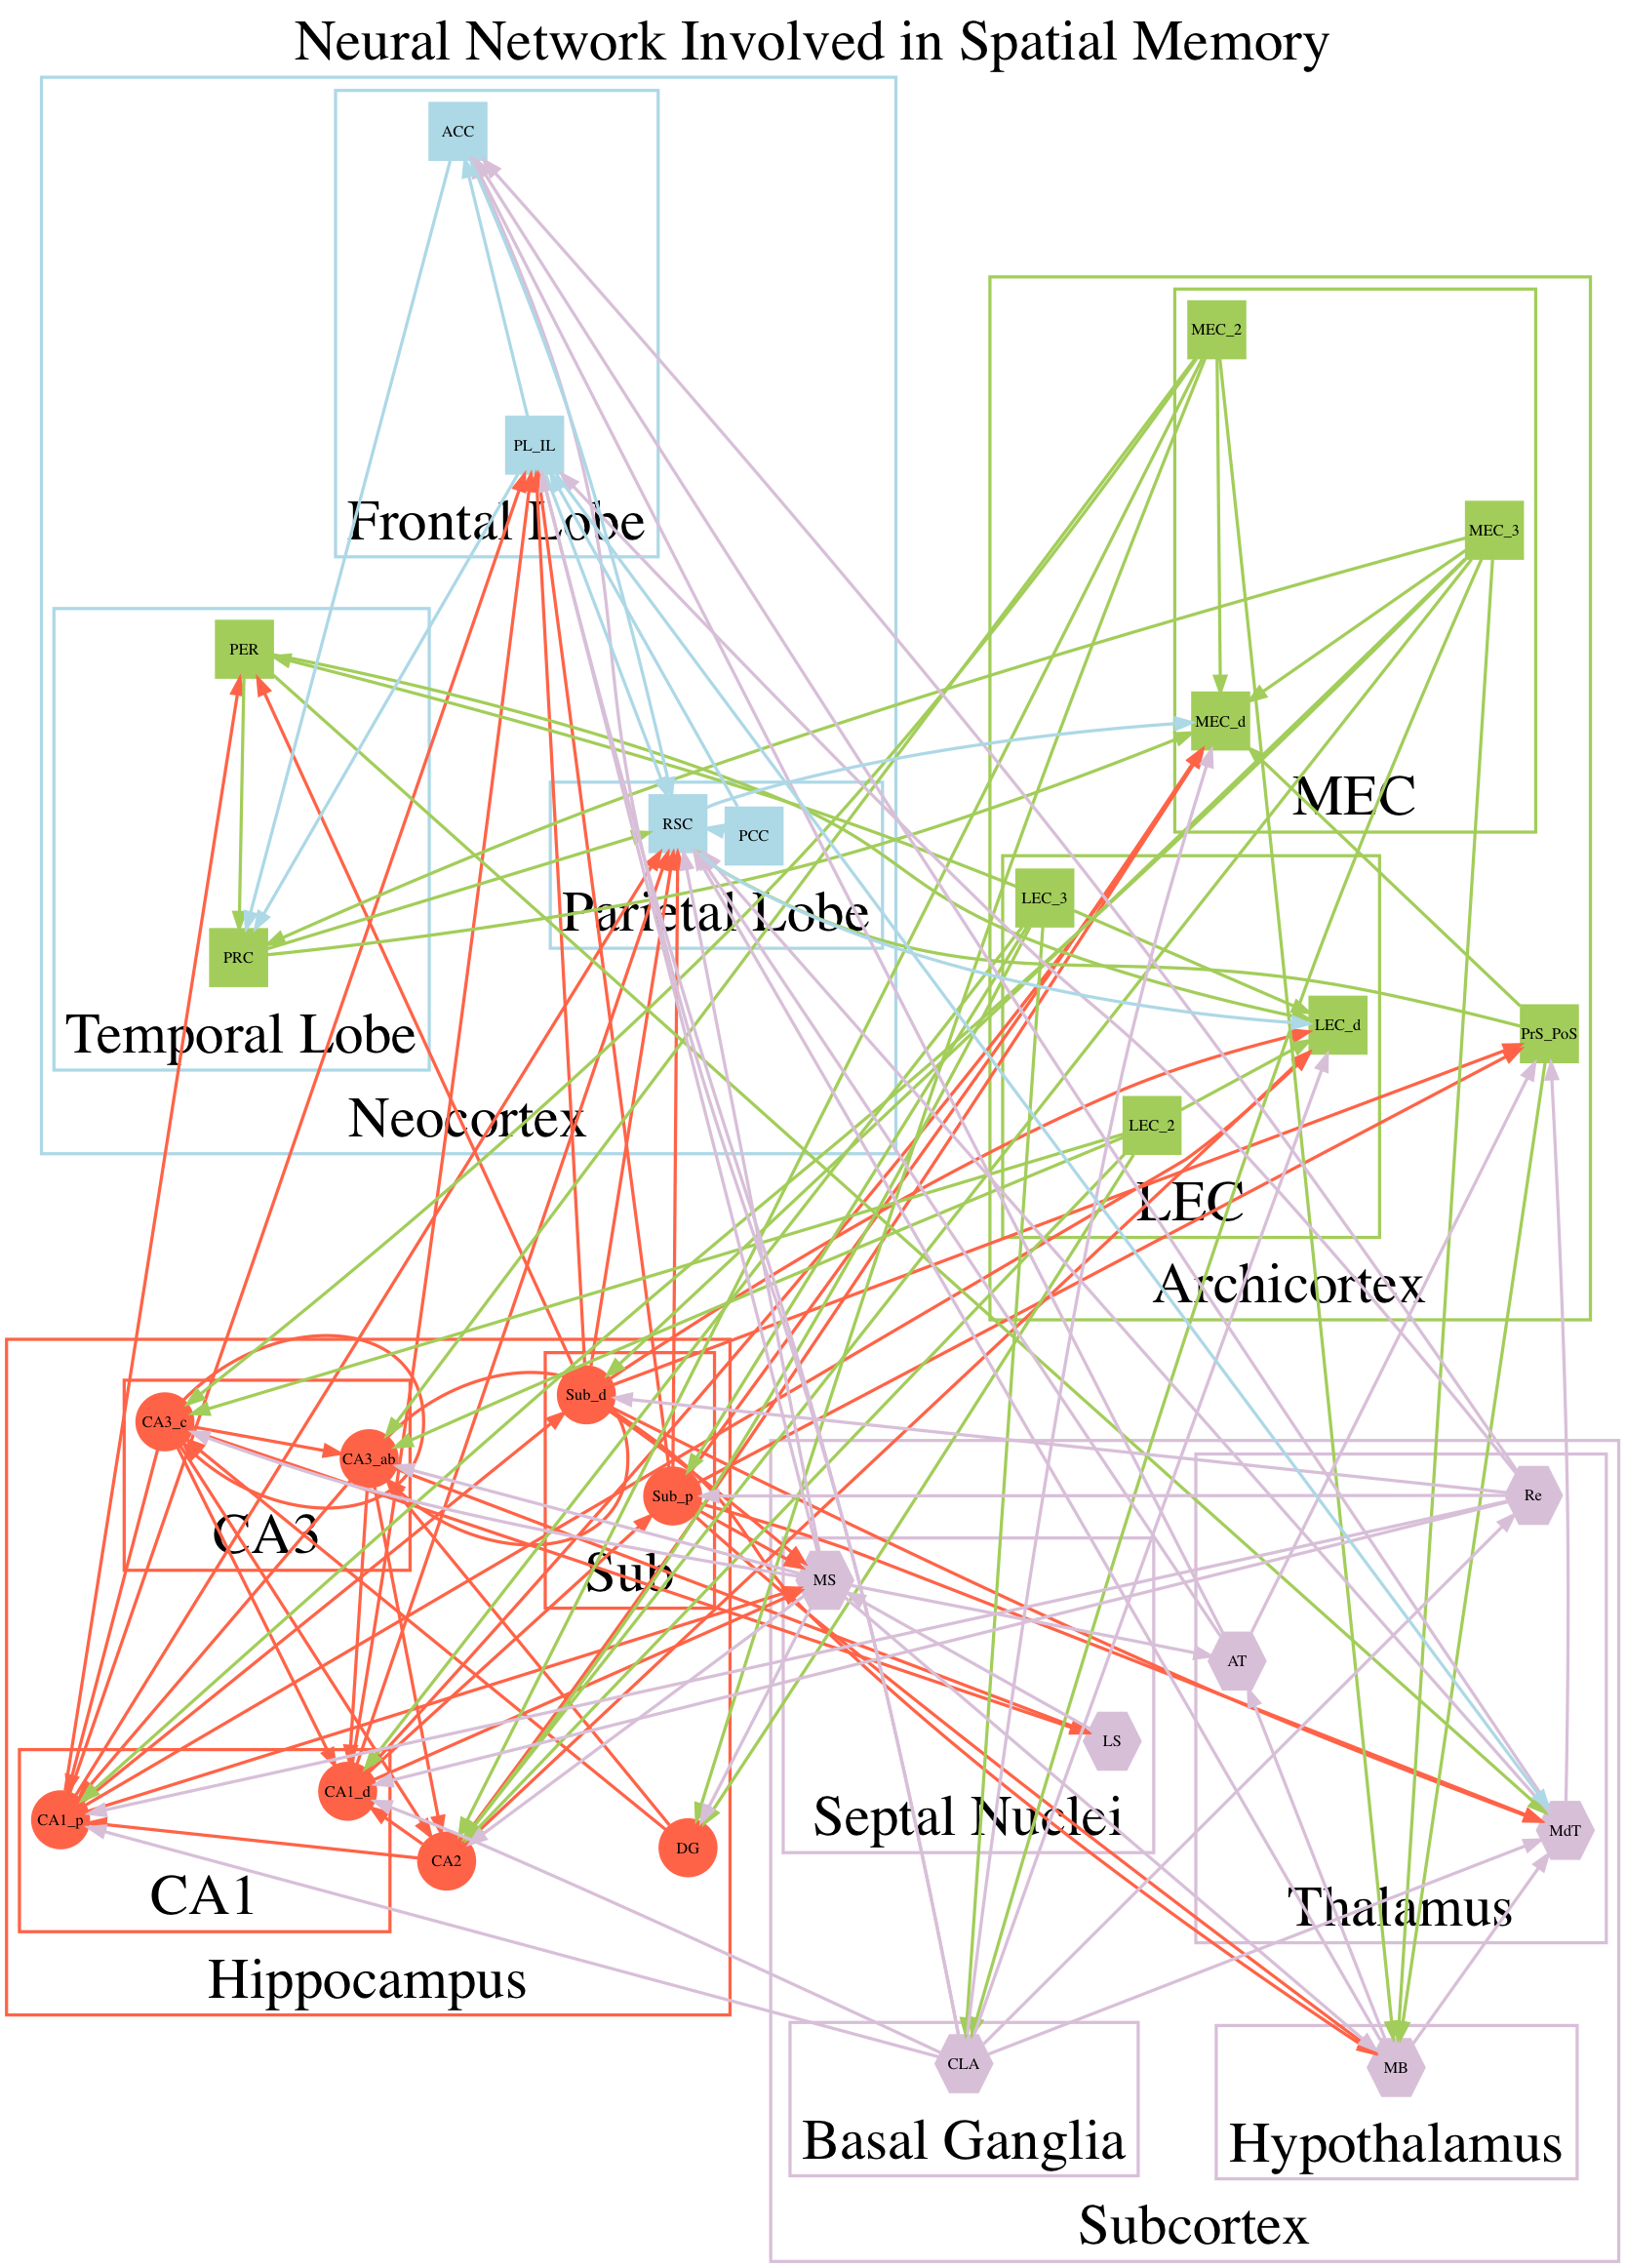
\includegraphics[width=.95\textwidth]{Complicated.png}
\begin{singlespace}
\caption {}
\end{singlespace}
\end{figure*}
\clearpage
\begin{figure*}
\captionsetup{labelformat=adja-page}
\ContinuedFloat
\caption{\textit{Model of spatial processing by interacting memory systems. This figure depicts an environment in which a rat is placed to explore in a spatial memory task \parencite{Goodrich-Hunsaker2005a, goodrich2008interactions}. For the event-based memory system with particular focus on the contributions from the hippocampus. Spatial relationships among stimuli are defined mathematically in terms of raw angles and distanced from the rat. For the knowledge-based memory system, spatial relationships are defined by only the most general geometric relationships (i.e., geometric shape defined by the elements-connectedness and neighbourhood), but without regard to the vantage of the rat for this processing or specific regard to which object is located at which node. The rule-based memory system uses affective information to guide exploratory behaviour and decisions undertaken by the rat. Importantly, the rule-based memory system can switch between the event- and knowledge-based memory systems as needed to guide behavioural performance. The final result is an active interaction among the three memory systems. We propose a role for the retrosplenial cortex in this integration. The retrosplenial cortex, having access to raw data from the thalamus, as well as the three memory systems, can perform computations in concert with the rule based memory system, as well as independently, and then signal that update to the rule-based memory system. Importantly, the retrosplenial cortex simplifies the spatial inputs to those relevant to guide task performance; this process provides a mechanism whereby an animal may compute egocentric position within an allocentric frame as proposed by other authors. Figure modified from \textcite{Hunsaker2013c} with permission }} \label{fig4}
\end{figure*}

The rule-based memory system sends projections into the elements processing the event-based and knowledge-based memory systems (\textit{i.e.}, PPC and hippocampus via entorhinal and parahippocampal cortices). Importantly, the retrosplenial cortex is in a unique location to integrate head direction information from the thalamus and subicular complex (pre/parasubiculum), metric/distal allocentric space from the hippocampus and event-based memory system and topologic/proximal egocentric space from the parietal cortex and knowledge-based memory system as well as reciprocal connectivity with the anterior cingulate, PL-IL cortices, agranular insula and rodent homologue to the dorsolateral prefrontal cortex. This allows the retrosplenial cortex to not only act upon incoming sensory information, but also to send the necessary signals to the rostral cortices to modulate/influence top down signals that guide behavior

This puts the retrosplenial cortex in a unique location to not only integrate the event and knowledge based memory systems or to compute egocentric location in allocentric space as has been proposed; but also to actively switch among pure egocentric, pure allocentric, and integrations involving combinations of the two-catered to the demands of each particular behavioral context.

The obvious benefit of having a structure in this location is that it allows full integration of multiple spatial reference frames in a manner that is capable of changing among many different states or forms depending upon the behavioral context. Additionally, it is likely that the retrosplenial cortex, in performing this integration removes redundancy from the spatial representation, which results in a parsimonious map sufficient to drive behavioral output, but not containing the resolution of the spatial map computed within the event-based memory system or elegant geometric representation of the knowledge-based memory system. Tasks requiring higher resolution metric information or demanding topological representations will result in the rule-based memory system biasing the integration to favor those modalities.

This is not a trivial point because the DG in the hippocampus will always compute an orthogonal representation of space based on a metric representations of distal cues and mathematical relationships among the local cues and the distal cues in relation to the location of the rodent, whether the behavioral situation demands such a map or not. In parallel, the parietal lobe will always compute a topological, or egocentric space with a particular focus on proximal cue configurations, even when doing so may be disruptive to performance of the behavioral or spatial task at hand. As such, neither the hippocampus nor parietal readout is sufficient to guide performance on behavioral tasks, even with the input from the rostral cortices with rule-based information, as neither the PPC nor the hippocampus contains or even has direct access to the others' spatial information.

Additionally, the retrosplenial cortex receives information pertaining to the sensory/perceptual and temporal attributes, as well as affective information via the PL-IL. This information from non-spatial attributes facilitate the identification of behavioral context, time of day or affective motivation; all information useful for the optimization of task performance.

The retrosplenial cortex, however, having a robust connectivity with both hippocampus, PL-IL, as well as parietal cortex, has relatively complete access to all types of information, as well as independently derived information pertaining to head direction from the thalamus and pre/parasubiculum (leading to retrosplenial neurons showing direction-based firing themselves). As such, with inputs from the PL-IL, the retrosplenial cortex can bias the integrated map toward topologic over metric information or ego over allocentric information as needed, or vice versa as situations demand. Additionally, the retrosplenial cortex can transmit information pertaining to the map being computed to the rostral cortices (esp. PL-IL, anterior insula and rodent homologue to the dorsolateral prefrontal cortex) to inform the rule based memory system pertaining to the maps being used to guide behavior.


\subsection{How to study interacting memory systems: Disconnection analyses}
It has been rather difficult to evaluate the specific roles for neural systems for learning and memory processes. Traditional lesion and inactivation experiments are useful for elucidating a functional role for a brain region of interest but as commonly employed are unable to provide information regarding a brain area's role in a larger neural network. Similarly, genetic manipulation of an animal may provide relatively good anatomical specificity, but again these methods do not allow the researcher to evaluate larger neural networks.

To partially overcome these weaknesses, a disconnection method can be employed. In this methodology, to determine whether two brain areas are interacting during performance of a particular behavior, two brain areas are unilaterally lesioned or inactivated. Since rodent brain function does not appear to be lateralized, if one unilaterally lesions or inactivates brain regions the animals by and large perform nominally on behavioral tasks. As such, one can lesion or inactivate two brain areas ipsilaterally as a control since the other hemisphere is intact. However, if a researcher inactivates two brain areas contralaterally, then the interaction between the two brain areas is inhibited, but the function of each brain region is preserved. In this way, disconnection analysis lets the researcher specifically probe whether an interaction among brain regions underlies task performance, or if both areas are independently involved. Table~\ref{tab1} provides a list of example disconnection studies used to elucidate the function of neural networks underlying processing within the spatial attribute. 

Moving forward, optogenetic techniques paired with single or multi-unit recording make it possible for researchers to actually determine a timescale for these interactions. As an example, it is still poorly understood at what timescale the retrosplenial cortex interacts with other brain areas. Is the retrosplenial cortex activated by the parietal cortex or does the retrosplenial cortex activate the parietal cortex during navigation tasks? The lesion and inactivation techniques reported in this manuscript lack the temporal precision to make these determinations. Using optogenetic and neurophysiological techniques it may be possible to determine which areas are involved earliest during a given memory process, and similarly it may be possible to determine the nature of information being output to areas activated later.

% BEGIN Table 1 
\begin{landscape}
\begin{longtable}{p{8cm}p{5cm}p{8cm}}
\caption{Selected example disconnection studies used to elucidate the function of neural networks underlying processing within the spatial attribute}\label{tab1} \\
\hline
Study & Brain Areas & Behavioral Task \\
\hline
\\
\endfirsthead
%
\multicolumn{3}{r}{-- continued from previous page} \\
\hline
Study & Brain Areas & Behavioral Task \\
\hline
\\
\endhead
			%
\hline \multicolumn{3}{r}{{Continued on next page}} \\ 
\hline
\endfoot
%
\hline
\endlastfoot
\cite{jo2010disconnection} & Hippocampus, \newline Perirhinal cortex & Object-placed paired association\\[20pt]
\cite{vann2011selective} & Hippocampus, \newline Mammillary bodies &Water Maze, \newline T Maze, \newline Radial arm maze\\[20pt]
\cite{churchwell2010prefrontal} & Agranular insula, \newline Prelimbic-Infralimbic, \newline CA1 & Modified Hebb-Williams maze\\[20pt]
\cite{dumont2010fornix} & Hippocampus, \newline Anterior thalamus, \newline Retrosplenial cortex & Object-context association\\[20pt]
\cite{wang2008reversible} & Prelimbic-Infralimbic, \newline Hippocampus&Water Maze, \newline Passive avoidance\\[20pt]
\cite{wang2006disconnection} & Prelimbic-Infralimbic, \newline Hippocampus & Delayed spatial alternation\\[20pt]
\cite{Rogers2007a} & Posterior parietal cortex, \newline Hippocampus & Object-place paired association, \newline Cheeseboard, \newline Spatial and nonspatial novelty detection\\[20pt]
\cite{jerman2006disconnection} & dDG, \newline dCA3 & Modified Hebb-Williams maze\\[20pt]
\cite{parron2006cooperation} & Hippocampus, \newline Entorhinal cortex & Water maze, \newline Spatial and nonspatial object recognition\\[20pt]
\cite{Lee2003} & PL-IL, \newline Hippocampus & Delay nonmatch to place on radial arm maze\\[20pt]
\cite{Warburton2001a} & Anterior thalamus, \newline Hippocampus & Water Maze, \newline T maze, Radial arm maze\\[20pt]
\cite{Warburton2000a} &Anterior thalamus, \newline Hippocampus & Water Maze, \newline T Maze, \newline Radial arm maze, \newline Object Recognition, \newline Spatial location recognition\\[20pt]
\cite{warburton1999does} & Anterior thalamus, \newline Hippocampus & Water maze\\[20pt]
\cite{neave1997evidence} & Cingulate cortex, \newline Hippocampus, \newline Mammillary Bodies & Delayed forced alternation, \newline Plus maze, \newline Radial arm maze, \\[20pt]
\cite{burcham1997disconnection} & Medial agranular cortex  \newline Posterior parietal cortex & Multimodal neglect\\[20pt]
\cite{warburton1998differential} & Anterior thalamus \newline Fornix & Water maze \\[20pt]
\cite{henry2004spatial} & Anterior thalamus \newline Hippocampus & spatial-visual conditional associative task \newline Delayed forced alternation\\[20pt]
\cite{barker2007recognition} & Prelimbic-Infralimbic \newline Perirhinal cortex & Object in place task \newline Object location\\[20pt]
\cite{ito2008functional} & Nucleus accumbens \newline Hippocampus & Appetitive spatial context conditioning \\[20pt]
\cite{vann2011selective} & Hippocampus \newline Mammillary bodies \newline Anterior Thalamus & Water maze \newline T maze \newline Radial arm maze\\[20pt]
\cite{chao2016medial} & Lateral entorhinal cortex \newline Prelimbic-Infralimbic & What-when-where task\\[20pt]
\cite{nelson2016importance} & Mammillary bodies \newline Anterior thalamus & Multiple item scene discrimination\\[20pt]
\cite{chao2017interaction} & Medial prefrontal cortex \newline CA1 & what-when-where task\\[20pt]
\cite{heimer2017disconnection} & Perirhinal cortex \newline Postrhinal cortex & Object in context recognition \newline Contextual fear conditioning \\[20pt]
\cite{OKADA2010295} & Entorhinal cortex, \newline Hippoampus & Spatial novelty detection\\[20pt]
\cite{HUNSAKER2009192}, \newline \cite{HUNSAKER2007127}, \newline \cite{hunsaker2009behavioral}, \newline \cite{HIPO:HIPO20429}, \newline \cite{HIPO:HIPO20288} & Hippocampus, \newline Lateral Septum, \newline Medial septum & Spatial novelty detection, \newline Modified Hebb-Williams maze, \newline Contextual fear conditioning, \newline Delay non-match to sample \\[20pt]
\cite{OLTON1982241} & Hippocampus, \newline Entorhinal cortex & Radial arm maze\\[20pt]
\cite{OLTON1978295} & Hippocampus, \newline Entorhinal cortex, \newline Lateral septum \newline Medial septum, \newline Mammillary bodies & Radial arm maze \\[20pt]
\cite{lassalle2000reversible} & CA3, \newline DG & Water maze\\[20pt]
\cite{floresco1997selective} & vCA1/vSubiculum, \newline Prelimbic-Infralimbic & Delay non-match to sample, \newline Random foraging \\[20pt]
\cite{Floresco11061}& Medial dorsal  thalamus, \newline Prelimbic-Infralimbic, \newline Nucleus accumbens & Delay and Nondelayed random foraging \\[20pt]
\cite{vann2013dismantling} & Hippocampus, \newline Mammillary bodies, \newline Gudden's ventral tegmental nucleus & Radial arm maze, \newline T-maze (allocentric and egocentric), \newline Water maze \\[20pt]
\cite{baker2014contralateral} & Prelimbic-Infralimbic, \newline Dorsomedial striatum & Cue signaled response shifting\\[20pt]
\cite{pecs1998lateralized} & CA1/CA3, \newline DG & Water maze\\[20pt]
\cite{dumont2015impact} & Hippocampus, \newline Anterior thalamus & Biconditional discrimination, \newline Passive place learing, \newline Spatial alternation, \newline Spatial Go-NoGo, \newline Spatial flexibility \\[20pt]
\cite{maren1997electrolytic} & Hippocampus, \newline Anterior thalamus & Contextual fear conditioning \\[20pt]
\cite{Vnek3193} & Hippocampus, \newline Entorhinal cortex & Acquisition and retention of object recognition\\[20pt]
\cite{trent2010ventral} & Lateral septum, \newline Ventral hippocampus & Elevated plus maze\\[20pt]
\cite{fu2016region} & PL-IL, \newline Dorsal CA1, \newline Ventral CA1, \newline Ventral DG & Auditory and Contextual fear conditioning \\[20pt]
\cite{dai2017contralateral} & PL-IL, \newline Hippocampus & W-maze spatial alternation\\[20pt]
\hline
\end{longtable}
\end{landscape}
%End Table 1

\printbibliography
\end{document}
